\def\anon{0} %Set to 1 for anonymous submissions, hides acknowledgements and author names
\def\full{1} %Set to 0 for springer proceedings

\ifnum\full=1
	\documentclass[11pt]{llncs}
	\addtolength{\parskip}{1pt}
\else
	\documentclass[10pt, runningheads]{llncs}
	\usepackage{times}
\fi



\usepackage{makeidx}
\usepackage[dvips]{graphicx}
\usepackage{graphicx}

\usepackage{comment}

\usepackage{listings}
\usepackage[mathscr]{eucal}
\usepackage{bm}
\usepackage{array}
\usepackage{url}
\usepackage{calc}
\usepackage{float}
\usepackage{latexsym}
\usepackage{rotating}
\DeclareGraphicsExtensions{.eps,.jpg,.png,.pdf}
%\usepackage[usenames, dvipsnames]{xcolor}
\usepackage[dvipsnames]{xcolor}
\usepackage[sort,nocompress]{cite}
\usepackage{colortbl}
\usepackage{multirow}
\usepackage{lscape}
\usepackage{amsmath}
\let\proof\relax
\let\endproof\relax
\usepackage{amsthm,amsfonts,amssymb}
\usepackage{hyperref}
\usepackage{pdflscape}


%\usepackage{natbib}

\def\rmdefault{ptm}

\usepackage{setspace}
\usepackage{color}
\ifnum\full=1
\usepackage[margin=0.9in]{geometry}
\usepackage{fullpage}

\setlength{\parskip}{0cm}

%\setstretch{1.03}
%\addtolength{\parskip}{1pt}
\setcounter{page}{0}
\renewcommand{\tabcolsep}{5pt}
\else
\renewcommand{\tabcolsep}{0pt}
\fi

\renewcommand{\arraystretch}{1.2}

\hyphenpenalty=5000
\tolerance=1000




%\ifnum\full=1
%\usepackage{natbib}
%\bibliographystyle{alpha}
%\setlength{\bibsep}{0pt}
%\renewcommand{\bibsection}{\section*{References}\small}
%\else
%\usepackage[numbers]{natbib}
%\bibliographystyle{splncs04}
%\fi



\DeclareMathOperator{\Exp}{E}
\DeclareMathOperator{\Var}{Var}
\DeclareMathOperator{\poly}{poly}
\DeclareMathOperator{\Supp}{Supp}

\usepackage{enumitem}


\usepackage{tikz}
\usetikzlibrary{arrows,shapes}
\usetikzlibrary{plotmarks}


%notes

%\definecolor{myorange}{rgb}{0.99,0.6,0.25}
%\newcommand{\pmnote}[1]{\colorbox{myorange}{\parbox{0.9\linewidth}{[{\footnotesize {\bf PM:} { {#1}}}]}}}


\definecolor{mycolor}{rgb}{0.75,0.95,0.05}
\newcommand{\pmnote}[1]{\colorbox{mycolor}{\parbox{0.9\linewidth}{[{\footnotesize {\bf PM:} { {#1}}}]}}}

\newcommand{\tsnote}[1]{\colorbox{orange}{\footnotesize\color{white}\textbf{TS: }#1}}

\definecolor{unmellowyellow}{rgb}{1.0, 1.0, 0.4}
\newcommand{\agnote}[1]{\colorbox{unmellowyellow}{\parbox{0.9\linewidth}{[{\footnotesize {\bf AG:} { {#1}}}]}}}
%% Sets

\newcommand{\Z}{\mathbb{Z}}
\newcommand{\N}{\mathbb{N}}
\newcommand{\R}{\mathbb{R}}
\newcommand{\C}{\mathbb{C}}
\newcommand{\F}{\mathbb{F}}
\newcommand{\Znm}{\mathbb{Z}_q^{n \times m}}

%matrices
\newcommand{\matzero}{\mathbf{0}}
\newcommand{\matA}{\mathbf{A}}
\newcommand{\matB}{\mathbf{B}}
\newcommand{\matC}{\mathbf{C}}
\newcommand{\matE}{\mathbf{E}}
\newcommand{\matF}{\mathbf{F}}
\newcommand{\matG}{\mathbf{G}}
\newcommand{\matI}{\mathbf{I}}
\newcommand{\matM}{\mathbf{M}}
\newcommand{\matP}{\mathbf{P}}
\newcommand{\matR}{\mathbf{R}}
\newcommand{\matS}{\mathbf{S}}
\newcommand{\matT}{\mathbf{T}}
\newcommand{\matU}{\mathbf{U}}
\newcommand{\matV}{\mathbf{V}}
\newcommand{\matW}{\mathbf{W}}
\newcommand{\matX}{\mathbf{X}}
\newcommand{\matY}{\mathbf{Y}}
\newcommand{\matZ}{\mathbf{Z}}


%vectors
\newcommand{\veca}{\mathbf{a}}
\newcommand{\vecb}{\mathbf{b}}
\newcommand{\vecc}{\mathbf{c}}
\newcommand{\vecd}{\mathbf{d}}
\newcommand{\vece}{\mathbf{e}}
\newcommand{\veci}{\mathbf{i}}
\newcommand{\vecj}{\mathbf{j}}
\newcommand{\veck}{\mathbf{k}}
\newcommand{\vecl}{\mathbf{l}}
\newcommand{\vecm}{\mathbf{m}}
\newcommand{\vecp}{\mathbf{p}}
\newcommand{\vecr}{\mathbf{r}}
\newcommand{\vecs}{\mathbf{s}}
\newcommand{\vecv}{\mathbf{v}}
\newcommand{\vecw}{\mathbf{w}}
\newcommand{\vecu}{\mathbf{u}}
\newcommand{\vecx}{\mathbf{x}}
\newcommand{\vecy}{\mathbf{y}}
\newcommand{\vecz}{\mathbf{z}}





%FiLIP notations

\newcommand{\FLIP}{\textsf{FLIP}}
\newcommand{\IFPl}{\text{Improved Filter Permutator} }
\newcommand{\IFPs}{\text{IFP} }

\newcommand{\FiLIP}{\textsf{FiLIP}}
\newcommand{\FiLIPDSM}{\mathsf{FiLIP}_{\mathsf{DSM}}}
\newcommand{\FiLIPXMAJ}{\mathsf{FiLIP}_{\mathsf{XMAJ}}}

%Boolean functions

\newcommand{\Bfn}[1]{\mathcal{B}_{#1}}
\newcommand{\BN}{\mathcal{B}_n}
\newcommand{\Bn}[1]{\mathcal{B}_{#1}}
\newcommand{\Bnstar}[1]{\mathcal{B}_{#1}^*}

\newcommand{\Bvad}[3]{\mathcal{B}({#1},{#2},{#3})}


\newcommand{\AI}{\mathsf{AI}}
\newcommand{\AN}{\mathsf{AN}}
%\newcommand{\difAN}[1]{\Delta_{\mathsf{AN}}(#1)}
%\newcommand{\DAN}{\mathsf{d}\mathsf{AN}}
%\newcommand{\Sd}{\mathsf{S}_\mathsf{d}}
\newcommand{\SD}{\mathsf{SD}}
\newcommand{\FAI}{\mathsf{FAI}}
\newcommand{\NL}{\mathsf{NL}}
\newcommand{\NLk}[1]{\mathsf{NL}_{#1}}
%\newcommand{\NLd}{\mathsf{NL_d}}
\newcommand{\res}{\mathsf{res}}
\newcommand{\bal}{\mathsf{bal}}
\newcommand{\gnlk}{\mathsf{GWNL}}


\newcommand{\DS}[1]{\mathsf{DS}(#1)}
\newcommand{\DSR}[2]{\mathsf{DS}^{#2}(#1)}
%\newcommand{\matAI}[3]{\mathbf{A}_{#2,#3}(#1)}

\newcommand{\WPB}[1]{\mathcal{WPB}_{#1}}
\newcommand{\WAPB}[1]{\mathcal{WAPB}_{#1}}
\newcommand{\SWAPB}[1]{\mathcal{SWAPB}_{#1}}
\newcommand{\SYM}[1]{\mathcal{SYM}_{#1}}
%for affine weightwise: degree and number of variables
\newcommand{\WD}[2]{\mathcal{WD}^{#1}_{#2}}
\newcommand{\Ekn}[2]{\mathsf{E}_{#1,#2}}
\newcommand{\Code}[2]{\mathsf{P}_{#1,#2}}
\newcommand{\mdist}[2]{\mathsf{d}_{#1,#2}}
%\newcommand{\Dka}[2]{\mathsf{D}_{#1}(#2)}
\newcommand{\Dnka}[3]{\mathsf{D}_{#1,#2}(#3)}

\newcommand{\dis}{\mathsf{c_1}}




\newcommand{\mnlk}[2]{\mu_{#1,#2}}
\newcommand{\Mnlk}[2]{\mathsf{M}_{#1,#2}}
\newcommand{\mnl}[1]{\mu_{#1}}
\newcommand{\Mnl}[1]{\mathsf{M}_{#1}}

\newcommand{\DistWkn}[2]{\mathfrak{W}_{#1,#2}}
\newcommand{\DistWn}[1]{\mathfrak{W}_{#1}}
\newcommand{\Dkn}[2]{\mathfrak{D}_{#1,#2}}
\newcommand{\Dn}[1]{\mathfrak{D}_{#1}}

\newcommand{\kraw}[3]{\mathsf{K}_{#1}(#2,#3)}
\newcommand{\phikn}[2]{\varphi_{#1,#2}}

\newcommand{\const}[2]{g_{#1,#2}}
\newcommand{\setn}[1]{S_{#1}}
\newcommand{\symsetsmall}[1]{A_{#1}}
\newcommand{\symset}[2]{B_{#1,#2}}


%usual notations
\newcommand{\supp}{\mathsf{supp}}
\newcommand{\suppk}[1]{\mathsf{supp}_{#1}}
\newcommand{\w}{\mathsf{w_H}}
\newcommand{\hd}{\mathsf{d_H}}
\newcommand{\degg}{\mathsf{deg}}
\newcommand{\Span}{\mathsf{Span}}
\newcommand{\rank}{\mathsf{rank}}
%Walsh transform
\newcommand{\wt}[1]{\mathcal W_{#1}} 
\newcommand{\Wsupp}[1]{\mathsf{Wsupp}_{#1}} 
%restricted Walsh transform W_k,a (f)
\newcommand{\wtk}[2]{\mathcal{W}_{#1,#2}} 

%S-equivalent classes
\newcommand{\sclass}[1]{\mathcal{S}(#1)}


\newcommand{\set}[1]{\left\{#1\right\}}
\newcommand{\mAN}[1]{\mathsf{d}_{#1}}


%gates
\newcommand{\AND}{\textsf{AND}}
\newcommand{\XOR}{\textsf{XOR}}
\newcommand{\MUX}{\textsf{MUX}}


%families of functions
\newcommand{\MAJ}{\textsf{MAJ}}
\newcommand{\DSM}{\textsf{DSM}}
\newcommand{\XORTHR}{\textsf{XOR-THR}}
\newcommand{\XORMAJ}{\textsf{XOR-MAJ}}

\newcommand{\xorlk}[2]{{\mathsf{XOR}}_{#1}  \mathsf{M}_{#2}} 
\newcommand{\xormaj}[2]{{\mathsf{XOR}}_{#1}  \mathsf{MAJ}_{#2}} 
%\newcommand{\xorthr}[3]{{\mathsf{XOR}}_{#1}  \mathsf{T}_{{#2},{#3}}} 
\newcommand{\xorthr}[3]{{\mathsf{XOR}}_{#1}+\mathsf{T}_{{#2},{#3}}}
\newcommand{\tri}[1]{{T}_{#1}}
\newcommand{\thr}[2]{\mathsf{T}_{{#1},{#2}}}
\newcommand{\xor}[1]{\mathsf{XOR}_{#1}}
\newcommand{\maj}[1]{\mathsf{MAJ}_{#1}}


\newcommand{\nbf}[1]{\mathsf{C}_{#1}}
\newcommand{\nbfodd}[2]{\mathsf{A}_{#1,#2}}
\newcommand{\nbfeven}[2]{\mathsf{B}_{#1,#2}}

%direct sum vector and simplified value vector
\newcommand{\dsv}[1]{\mathbf{m}_{#1}}
\newcommand{\svv}[1]{\mathbf{s}_{#1}}

% Define a custom theorem style for bold optional arguments
\newtheoremstyle{boldoptional} % Name of the style
  {3pt}                        % Space above
  {3pt}                        % Space below
  {\itshape}                   % Body font
  {}                           % Indent amount
  {\bfseries}                  % Theorem head font
  {.}                          % Punctuation after theorem head
  { }                          % Space after theorem head
  {\thmname{#1}\thmnumber{ #2}\thmnote{ (\textbf{#3})}} % Bold optional argument

% Apply the new style to Property
\theoremstyle{boldoptional}
\newtheorem{Prop}{Property}
\newtheorem{Cons}{Construction}


% For algorithms
\usepackage{algorithm,algpseudocode}

\renewcommand{\algorithmicrequire}{\textbf{Input:}}
\renewcommand{\algorithmicensure}{\textbf{Output:}}
% \renewcommand{\ALG@name}{Construction}
\newenvironment{constr}[1][htb]{%
\floatname{algorithm}{Construction}% Update algorithm name
   \begin{algorithm}[#1]%
  }{\end{algorithm}}
 
\algnewcommand\algorithmicparfor{\textbf{par-for}}
\algdef{S}[FOR]{ParFor}[1]{\algorithmicparfor\ #1\ \algorithmicdo}
 
%latin

\newcommand{\ie}{\textit{i.e.}}
\newcommand{\eg}{\textit{e.g.}}
\newcommand{\ea}{\textit{et al.}}

%Tim's stuff
\newtheorem{Corollary}{Corollary}
\newcommand{\ii}{\mathrm i\mkern1mu} %Imaginary unit
\newcommand{\ee}{\mathrm e\mkern1mu} %Euler constant
\newcommand{\dd}{\,\mathrm d} %Differential
\newcommand{\ui}[1]{^{(#1)}} %Upper index
\newcommand{\mycomment}[1]{} %Comment out entire parts
\usepackage{mleftright}
\mleftright %Less space when using \left and \right


\newcommand{\tablecaption}[1]{%
   \vspace{3pt} % Adds space above the caption
   \caption{#1} % Displays the caption text
}

\let\leq=\leqslant %Replace symbol for \leq
\let\geq=\geqslant %Replace symbol for \geq

\newcommand{\hwbf}{\textsf{HWBF}}

%No line break before lists
\makeatletter
\@beginparpenalty=10000
\makeatother

\begin{document}

\setcounter{page}{1}

\title{The Revisited Hidden Weight Bit Function}
\titlerunning{The Revisited Hidden Weight Bit Function}

\ifnum\anon=0
	\author{%
		Pierrick M\'eaux\inst{1},
		Tim Seuré\inst{1}, 
		Deng Tang\inst{2}
		%Pierrick M\'eaux\orcidID{0000-0001-5733-4341}\inst{1},
		%Tim Seuré\inst{1}, 
		%Deng Tang\orcidID{0000-0002-8373-9200}\inst{2}
	}
	\authorrunning{P.\ M\'eaux, T.\ Seur\'e, D.\ Tang}
	\institute{%
		University of Luxembourg, Luxembourg\\
		\email{pierrick.meaux@uni.lu, tim.seure@uni.lu} 
		\and
		Shanghai Jiao Tong University, Shanghai, China\\
		\email{dengtang@sjtu.edu.cn}
	}
\else
	\author{}
	\institute{}
\fi

\maketitle	
	
\begin{abstract}
	The Hidden Weight Bit Function (\hwbf{}) has drawn considerable attention for its simplicity and cryptographic potential. 
	Despite its ease of implementation and favorable algebraic properties, its low nonlinearity limits its direct application in modern cryptographic designs. In this work, we revisit the \hwbf{} and propose a new weightwise quadratic variant obtained by combining the \hwbf{} with a bent function. 
	This construction offers improved cryptographic properties while remaining computationally efficient. We analyze the balancedness, nonlinearity, and other criteria of this function, presenting theoretical bounds and experimental results to highlight its advantages over existing functions in similar use cases. The different techniques we introduce to study the nonlinearity of this function also enable us to bound the nonlinearity of a broad family of weightwise quadratic functions, both theoretically and practically. We believe these methods are of independent interest.

	\keywords{Boolean functions, HWBF, Nonlinearity.}
\end{abstract}

\section{Introduction}

The Hidden Weight Bit Function (\hwbf{}) has attracted significant attention since its introduction by Bryant in 1991~\cite{IEEE:Bryant91}. It has been regarded as the simplest example of a function whose binary decision diagram has exponential size~\cite{IEEE:Bryant91,TIA:BoLSW99}. The ease of implementing this function across various computational models—owing to its reliance on computing the Hamming weight of the input and applying a simple linear function—combined with its relatively strong cryptographic properties as demonstrated in~\cite{DAM:WCST14} (\eg, balancedness, nonlinearity, degree, and algebraic immunity), has made it a noteworthy candidate for use as a filter function in stream cipher constructions.

Recent developments in stream ciphers have reignited interest in this function. The emergence of new applications for stream ciphers with filter functions on a larger number of variables—such as Hybrid Homomorphic Encryption (\textsf{HHE})~\cite{CCS:NaeLauVai11}—has further emphasized the relevance of such functions. \textsf{HHE} requires Boolean functions that can be efficiently evaluated in an input-oblivious algorithm. For instance, several new binary stream ciphers have been proposed since 2016, including Kreyvium~\cite{JOC:CCFLNP18}, \textsf{FLIP}~\cite{EC:MJSC16}, Rasta~\cite{C:Rasta}, \textsf{FiLIP}~\cite{INDO:MCJS19}, Dasta~\cite{TOSC:BeiLea20} and Fasta~\cite{CTRSA:CidIndRad22}. 
Currently, designs employing Boolean functions with more than one hundred variables as filters lead to \textsf{HHE} schemes with the best latency~\cite{INDO:HofMeaRic20,CCS:CDPP22,CIC:MeaParPei24,eprint:AGHM24}.

The \hwbf{}, while efficient to compute, suffers from low nonlinearity, which limits its direct application as a filter function. Consequently, various generalizations have been explored to enhance this parameter while preserving or improving other cryptographically relevant properties, such as balancedness, algebraic degree, and algebraic immunity. Notable examples include functions introduced in~\cite{IEEE:Carlet22,eprint:CarPar23} and~\cite{DAM:MeaOza24}. The latter work considers functions obtained by computing the Hamming weight of the input and applying a quadratic Boolean function, so-called weightwise quadratic functions.

\bigskip

In this article, we propose a new generalization of the \hwbf{}, a weightwise quadratic function constructed by \textsf{XOR}-ing the \hwbf{} with a bent quadratic function. This leads to a family of Boolean functions that are computationally efficient and feature superior cryptographic properties compared to previous constructions. 
Additionally, the techniques we introduce to analyze nonlinearity have broader applicability and provide bounds on the maximum absolute Walsh spectrum for a wider class of weightwise quadratic functions. Our contributions are as follows:

\begin{itemize}
	\item\emph{Balancedness analysis} (Section~\ref{sec:defAndBal}): We define the revisited \hwbf{} in $n$ variables, hereafter denoted by $f$, and analyze its balancedness. This involves studying the (restricted) Walsh transform of specific quadratic functions over sets of fixed Hamming weights (called slices). By establishing recursive relations for these values, we determine for which values of $n$ the function is balanced.
    \item \emph{Nonlinearity bounds} (Section~\ref{sec:dnk}):
    We relate the maximum Walsh coefficients of the revisited \hwbf{} to the coefficients of generating functions and employ complex analysis techniques to prove lower bounds on the nonlinearity of $f$. 
    Unlike most studies on Boolean functions used in cryptography, this approach yields strong nonlinearity bounds for a broader class of functions in an even number of variables.
    \item \emph{Experimental results and comparisons} (Section~\ref{sec:expAndComp}): 
    For bounded values of $n$, we employ specific techniques to refine the nonlinearity bounds of $f$, providing tighter estimates up to $n = 80$. Through experiments, we compare these bounds with actual nonlinearity values for $f$ and other weightwise quadratic functions, such as the majority function, the \hwbf{}, and the two main examples in~\cite{DAM:MeaOza24}. 
    Our results highlight the revisited \hwbf{}'s superior nonlinearity relative to functions with similar computational costs.
    \item \emph{Analysis of other cryptographic parameters} (Section~\ref{sec:otherParameters}):  
    We evaluate other cryptographically relevant parameters of $f$, including degree, algebraic immunity, and fast algebraic immunity. Similar to the nonlinearity analysis, the revisited \hwbf{} outperforms or matches other functions with comparable computational costs.
\end{itemize}

\section{Preliminaries}

Throughout this paper, $n\geq 0$ will always denote a non-negative integer. Further, our intervals will only contain integers, so that for instance $[0,n]=\{0,1,\dots,n\}$. The set of binary vectors of length $n$ will be denoted by $\F_2^n$, with the zero vector written as $0_n$. The canonical basis of $\F_2^n$ will be written as $\{e_1,\dots,e_n\}$; therefore, $e_i\in\F_2^n$ is the vector which is zero everywhere except at position $i$. The entries of a binary vector $x\in\F_2^n$ will always be denoted by $x_1,\dots,x_n$. Given a permutation $\pi:[1,n]\to[1,n]$ and a vector $x\in\F_2^n$, we define $\pi(x)=(x_{\pi(i)})_{i\in[1,n]}\in\F_2^n$. We write the scalar product of two binary vectors $x,y\in\F_2^n$ as $x\cdot y=\sum_{i=1}^nx_iy_i\in\F_2$. The Hamming weight of a binary vector $x\in\F_2^n$ is denoted by $\w(x)=|\{i\in [1,n]:x_i=1\}|$.

\subsection{Boolean functions and cryptographic parameters}

In this part, we recall general concepts on Boolean functions and their cryptographic properties we use in this article. 
For a deeper introduction on Boolean functions and their cryptographic parameters, we refer to the book~\cite{Carlet20}, and to~\cite{TOSC:CarMeaRot17} for properties on slices, so-called weightwise properties.

\begin{definition}[Slice]
    For any integer $k$, we introduce the set $\Ekn{k}{n}=\{x\in \F_2^n:\w(x)=k\}$, and call it the $k$-th slice of the Boolean hypercube (of dimension $n$); note that if $k\not\in[0,n]$, then $\Ekn kn=\varnothing$.
\end{definition}

\begin{definition}[Boolean function]\label{def:bool_f}
	A Boolean function in $n$ variables is a function from $\F_2^n$ to $\F_2$. The set of all Boolean functions in $n$ variables is denoted by $\BN$, and we denote this set without the null function by~$\BN^*$.
\end{definition}

Below, for a Boolean function $f\in\BN$, we write $f+1$ for the Boolean function $g\in\BN$ which satisfies $g(x)=f(x)+1$ for every $x\in\F_2^n$.

\begin{definition}[Algebraic Normal Form, degree]\label{def:anf}
	We call Algebraic Normal Form of a Boolean function $f\in\BN$ its unique representation as an element of the ring $\F_2[x_1,\dots,x_n]/(x_1^2+x_1,\dots,x_n^2+x_n)$, and we express it as follows:
	\[
		f(x_1,\dots,x_n)= \sum_{I \subseteq [1,n]} a_I \left( \prod_{i \in I} x_i \right),
	\]
	where $a_I\in \F_2$. The (algebraic) degree of $f$ is defined by $\degg(f)=0$ in case $f$ is the null function, and $\degg(f)=\max\{ |I|:I\subseteq[1,n],a_I=1\}$ otherwise.
\end{definition}

\begin{definition}[Walsh transform, restricted Walsh transform]\label{def:walsh_transform}
	The Walsh transform at $a \in \F_2^n$ of a Boolean function $f\in\BN$ restricted to a subset $S\subseteq \F_2^n$ is defined as:
    \[  \wt{f,S} (a) = \sum_{x\in S} (-1)^{f(x)+a \cdot x}.\]
    The (unrestricted) Walsh transform of $f$ is then defined as $\wt{f}=\wt{f,\F_2^n}$. For any integer $k$, we also set $\wt{f,k}=\wt{f,\Ekn{k}{n}}$.
\end{definition}

\begin{definition}[Balancedness]
%    A Boolean function $f\in\BN$ is called balanced if $\wt f(0_n)=0$.
A Boolean function $f\in\BN$ is called balanced if $|\{x \in \F_2^n : f(x)=0\}|=2^{n-1}=|\{x \in \F_2^n : f(x)=1\}|$. 
Equivalently, $f$ is balanced if and only if $\wt f(0_n)=0$.
\end{definition}

\begin{definition}[Nonlinearity, \eg, page 79 in \cite{Carlet20}]%and weightwise nonlinearity
	\label{def:nl}
	The nonlinearity $\NL(f)$ of a Boolean function $f\in \BN$ is the minimum Hamming distance between $f$ and all the affine functions in $\BN$:
	\[
		\NL(f) = \min\{ \hd(f,g):g\in\BN,\degg(g)\leq 1\},
	\]
	where the Hamming distance between $f$ and $g$ is defined as $\hd(f,g)=|\{x\in\F_2^n:f(x)\neq g(x)\}|$. Alternatively, the nonlinearity of $f\in\BN$ can also be defined in terms of its Walsh transform:
	\[
		\NL(f) = 2^{n-1}- \frac{1}{2} \max_{a\in \F_2^n}{|\wt{f}(a)|}.
	\]
\end{definition}

When $n$ is even, the nonlinearity of a Boolean function in $n$ variables can reach at most $2^{n-1}-2^{n/2 -1}$. Functions reaching this maximum are called bent functions. Due to their broad applications and importance, they have been the focus of multiple works, \eg, \cite{Rothaus76,FSE:Dobbertin95,DBLP:conf/itw/BudaghyanCH11,Tokareva15,Mesnager16}. 
The quadratic function $d_n\in\BN$ given by $d_n(x)=\sum_{i=1}^{n/2}x_{2i-1}x_{2i}$ is an example for such a bent function.

\bigskip

The algebraic degree of multiples of a Boolean function is a crucial quantity for various attacks on stream ciphers that utilize a Boolean function as a filter. 
The well-known algebraic attack~\cite{EC:CouMei03} and fast algebraic attack~\cite{C:Courtois03} on filtered \textsf{LFSR}s have motivated the study of cryptographic properties such as algebraic immunity and fast algebraic immunity, \eg, \cite{FSE:Armknecht04,C:HawRos04,ISC:JiaZhaWan13}. Nowadays, these parameters are systematically determined for any function considered as a filter.

\begin{definition}[Annihilator, algebraic immunity~\cite{EC:MeiPasCar04}] \label{def:ai}
	Let $f\in\BN$ be a Boolean function. Then a function $g\in\BN^*$ is called an annihilator of $f$ if it satisfies $fg=0$. The algebraic immunity of $f$ is then defined as:
	\[ \AI(f) = \min\{ \degg(g):\text{$g\in\BN^*$ is an annihilator of $f$ or $f+1$}\}.\]
\end{definition}

\begin{definition}[Fast algebraic immunity, \eg, \cite{EC:ACGKMR06,IEEE:LiuLinPei11,DCC:CarTan15}]\label{def:FAI}
	The fast algebraic immunity of a Boolean function $f\in \Bfn{n}$ is defined as:
	\[
		\FAI(f)=\min \{ 2 \AI(f), \min\{\degg(g)+ \degg(fg):g\in\BN,1\leq\degg(g)<\AI(f)\}\}.
	\]
\end{definition}

\subsection{Symmetric Functions, \hwbf{} and weightwise degree-$d$ functions}

Recall that the Boolean symmetric functions in $n$ variables are those that are constant on the slice $\Ekn{k}{n}$ for every $k\in [0,n]$. 
This class of functions has been thoroughly studied in the context of cryptography, see \eg, \cite{IEEE:Carlet04,IEEE:CanVid05,INDO:BraPre05,DM:SarMai07,IEEE:QFLW09,IEEE:CheLu11,Latin:Meaux19,CCDS:Meaux21,IEEE:CarMea21}.
In this article, the symmetric functions that we consider will mainly be the slice indicator function and the majority function.

\begin{definition}[Slice indicator functions]\label{def:slice}
	The indicator function of the slice of weight $k\in[0,n]$ is the function $\phikn kn\in\BN$ defined by $\phikn kn(x)=1$ if and only if $\w(x)=k$.
\end{definition}

\begin{definition}[Majority function]\label{def:maj}
    The majority function in $n$ variables is the Boolean function $\mathsf{Maj}_n\in\BN$ defined by $\mathsf{Maj}_n(x)=1$ if and only if $\w(x)\geq n/2$.
\end{definition}

Bigger families of functions can be obtained by considering functions of bounded degree on each slice. This corresponds to the concept of weightwise degree-$d$ functions introduced in~\cite{DAM:GinMea22} for $d=1$ and~\cite{DAM:MeaOza24} for the general case. 

\begin{definition}[Weightwise degree-\textit{d} functions, Definition 12 in \cite{DAM:MeaOza24}]\label{def:wwdegd}
    A Boolean function $f\in\BN^*$ is called weightwise degree-$d$ if it can be written under the form $f=\sum_{k=0}^n f_k \phikn{k}{n}$ with $f_k\in\BN$ of degree at most $d$. The set of weightwise degree-$d$ functions is denoted by $\WD{d}{n}$.
	Additionally, a weightwise degree-$d$ function $f=\sum_{k=0}^n f_k \phikn{k}{n}$ is called a cyclic weightwise degree-$d$ function if for all $k\in [0,n]$ and all $x\in\F_2^n$, it holds that $f_k(x)=f_0(O^k(x))$, where $O^k:\F_2^n\to\F_2^n$ is the cyclic shift by $k$ positions, defined by $O^k(x_1,\dots,x_n)=(x_{(1+k)\bmod n},\dots,x_{(n+k)\bmod n})$, the representatives modulo $n$ being taken as integers in $[1,n]$.
\end{definition}

Various weightwise affine functions (\ie, belonging to $\WD{1}{n}$) have been exhibited, such as in~\cite{TOSC:CarMeaRot17} where the bent functions in Propositions $1$ and $2$ are weightwise affine, or in~\cite{DAM:GinMea22} to show than no weightwise perfectly balanced function is weightwise affine for $n\geq 8$. 
The arguably best known example of weightwise affine function is the Hidden Weight Bit Function introduced in~\cite{IEEE:Bryant91}, the one obtained by fixing $f_0=0$ and $f_k=x_k$ for $k \in [1,n]$. The cryptographic properties of this function have been studied in~\cite{DAM:WCST14}, showing good algebraic properties for this function.

\begin{definition}[Hidden Weight Bit Function]\label{def:hwbf}
    We call Hidden Weight Bit Function (\hwbf{}) the Boolean function $h\in\BN$ defined as:
	\[
		h(x)=\sum_{k=1}^{n}x_k\phikn{k}{n}(x).
	\]
\end{definition}

In~\cite{DAM:MeaOza24}, the parameters of different functions from $\WD{1}{n}$ and $\WD{2}{n}$ are studied experimentally for $n$ up to $20$, and lower bounds are given for the nonlinearity for all $n$. 
These bounds focus on cyclic weightwise quadratic functions and involve sums of binomial coefficients. For simplicity, in the following we provide only the nonlinearity values of the majority function and \hwbf{}, as these bounds will be used for comparison.

\begin{Prop}\label{prop:wwd1}
	Let $n\geq 2$ be an even integer.
	\begin{itemize}
		\item (\eg, Theorem $3$ in~\cite{DCC:DalMaiSar06}) The majority function $\mathsf{Maj}_n$ introduced in Definition~\ref{def:maj} satisfies:
		\[
			\NL(\mathsf{Maj}_n)=2^{n-1}-\binom{n-1}{\frac n2}.
		\]
		\item (Theorem $3$ in~\cite{DAM:WCST14}) The \hwbf{} $h$ introduced in Definition~\ref{def:hwbf} satisfies:
		\[
			\NL(h)=2^{n-1}-2\binom{n-2}{\frac{n-2}{2}}.
		\]	
		\item (Theorem $1$ in \cite{DAM:WCST14}) The \hwbf{} $h$ introduced in Definition~\ref{def:hwbf} satisfies $\degg(h)=n-1$ if $n\geq 4$.
	\end{itemize}
\end{Prop}

\subsection{Krawtchouk polynomials}

We use Krawtchouk polynomials and some of their properties to prove one of our main results. We give the necessary definition here and refer to \cite{book:MacSlo78} for more details, for instance.

\begin{definition}[Krawtchouk polynomials]\label{def:Kraw}
	The $n$-th Krawtchouk polynomial of degree $k\in\Z$ is given by:
    \[
        \kraw{k}{x}{n}=\sum_{j=0}^{k} (-1)^j \binom{x}{j} \binom{n-x}{k-j}.
    \]
    The Krawtchouk polynomials can alternatively be characterized as the coefficients in the generating function for $(1+z)^{n-x} (1-z)^x$ in the variable $z$:
    \[
        (1+z)^{n-x} (1-z)^x=\sum_{k\in\Z} \kraw{k}{x}{n} z^k.
    \]
\end{definition} 

\section{Revisited \hwbf{} and balancedness}\label{sec:defAndBal}

In this part, we will formally define the revisited \hwbf{} function and introduce a quantity that allows us to study its balancedness and nonlinearity.

\begin{definition}[Revisited \hwbf{}]\label{def:revHWBF}
	For an even integer $n\geq 0$, we call revisited \hwbf{} the Boolean function $f\in\BN$ defined as:
	\[
		f(x)=\sum_{k=1}^nx_k\phikn{k}{n}(x)+\sum_{i=1}^{n/2}(x_i+1) x_{i+n/2}.
	\]
\end{definition}

Since $f$ is the sum of a quadratic function and a weightwise affine function, it is a weightwise quadratic function. Using the formalism of Definition~\ref{def:wwdegd}, $f$ is the weightwise quadratic function defined by $f_0(x)=0$ and $f_k(x)=x_k+\sum_{i=1}^{n/2}(x_i+1) x_{i+n/2}$ for $k\in[1,n]$. This form allows to derive the restricted Walsh transform of $f$, which can be a useful tool to study the balancedness and bound the nonlinearity of a function.

\begin{proposition}\label{prop:restrWT}
	Let $n\geq 0$ be an even integer, and let $f\in\BN$ be the revisited \hwbf{}. Consider any binary vector $a\in\F_2^n$ and any integer $k\in[1,n]$. Define $c=a+e_k+\sum_{i=n/2+1}^n e_i$. Then the restricted Walsh transform of $f$ satisfies:
	\[
		\wtk{f}{k}(a)=\sum_{x \in \Ekn{k}{n}} (-1)^{\sum_{i=1}^{n/2} x_i x_{i+n/2}+ c \cdot x}.
	\]
\end{proposition}

\begin{proof}
	We compute:
	\begin{align*}
		\wtk{f}{k}(a)&=\sum_{x \in \Ekn{k}{n}} (-1)^{f(x)+a \cdot x}\\
		&=\sum_{x \in \Ekn{k}{n}} (-1)^{x_k + \sum_{i=1}^{n/2} (x_i+1) x_{i+n/2}+ a \cdot x}\\
		&=\sum_{x \in \Ekn{k}{n}} (-1)^{\sum_{i=1}^{n/2} x_i x_{i+n/2}+\left(x_k+\sum_{i=n/2+1}^{n}x_i+a\cdot x\right)}\\
		&=\sum_{x \in \Ekn{k}{n}} (-1)^{\sum_{i=1}^{n/2} x_i x_{i+n/2}+ c \cdot x}.\qedhere
	\end{align*}
\end{proof}

Accordingly, we can study the restricted Walsh transform of the revisited \hwbf{} by analyzing the one of the following Boolean function $d_n\in\BN$.

\begin{definition}
	Let $n\geq 0$ be an even integer. Then we define the Boolean function $d_n\in\BN$ by:
	\[
		d_n(x)=\sum_{i=1}^{n/2}x_{2i-1}x_{2i}.
	\]
	Further, for an integer $k$ and a binary vector $a\in\F_2^n$, we define:
	\[
		\Dnka{n}{k}{a}=\wtk{d_n}{k}(a)=\sum_{x\in \Ekn{k}{n}} (-1)^{d_n(x) +a\cdot x}.
	\]
\end{definition}

The $\Dnka{n}{k}{a}$ satisfy a recursive relation.

\begin{proposition}\label{prop:recursiveDnka}
Let $n\geq 0$ be an even integer. Then for all integers $k$ and all binary vectors $a\in\F_2^n$, the following hold true:
	\begin{itemize}
		\item We have $\Dnka 00a=1$ and $\Dnka 0ka=0$ if $k\neq 0$.
		\item If $n\geq 2$, then for $b=(a_1,\dots,a_{n-2})\in\F_2^{n-2}$, we have:
		\[
			\Dnka{n}{k}{a}=\Dnka{n-2}{k}{b}+\left((-1)^{a_{n-1}} + (-1)^{a_{n}}\right)\Dnka{n-2}{k-1}{b} + (-1)^{1+a_{n-1}+a_n} \Dnka{n-2}{k-2}{b}.
		\]
	\end{itemize}
\end{proposition}

\begin{proof}
    We have that $\Dnka 00a=(-1)^0=1$ since $\Ekn 00=\{\varepsilon\}$ for the empty vector $\varepsilon=a\in\F_2^0$. That $\Dnka 0ka=0$ if $k\neq 0$ follows from $\Ekn k0$ being empty if $k\neq 0$. Assume now that $n\geq 2$. By considering binary vectors $x\in\F_2^n$ as $x=(y,x_{n-1},x_n)$ for $y\in\F_2^{n-2}$, we get:
    \begin{align*}
		\Dnka{n}{k}{a}&=\sum_{x\in \Ekn{k}{n}} (-1)^{d_n(x) +a\cdot x}\\
		&=\sum_{y\in \Ekn{k}{n-2}} (-1)^{d_{n-2}(y) +b\cdot y}+
		\sum_{y\in \Ekn{k-1}{n-2}} (-1)^{d_{n-2}(y) +b\cdot y + a_{n-1}}\\
		&\qquad+\sum_{y\in \Ekn{k-1}{n-2}} (-1)^{d_{n-2}(y) +b\cdot y + a_{n}}
		+\sum_{y\in \Ekn{k-2}{n-2}} (-1)^{d_{n-2}(y) +b\cdot y +1 + a_{n-1}+ a_{n}}\\
		&=\Dnka{n-2}{k}{b}+\left((-1)^{a_{n-1}} + (-1)^{a_{n}}\right)\Dnka{n-2}{k-1}{b} + (-1)^{1+a_{n-1}+a_n} \Dnka{n-2}{k-2}{b}.\qedhere
    \end{align*}
\end{proof}

\begin{remark}
    We note that Proposition~\ref{prop:recursiveDnka} gives three different cases depending on the values of the two last elements of $a$:%Then it gives three cases:
	\begin{itemize}
		\item if $a_{n-1}=0=a_n$, then $\Dnka{n}{k}{a}=\Dnka{n-2}{k}{b}+2\Dnka{n-2}{k-1}{b}-\Dnka{n-2}{k-2}{b}$,
		\item if $a_{n-1} \ne a_n$, then $\Dnka{n}{k}{a}=\Dnka{n-2}{k}{b}+\Dnka{n-2}{k-2}{b}$,
		\item if $a_{n-1}=1=a_n$, then $\Dnka{n}{k}{a}=\Dnka{n-2}{k}{b}-2\Dnka{n-2}{k-1}{b}-\Dnka{n-2}{k-2}{b}$.
	\end{itemize}
\end{remark}

\begin{remark}\label{rmk:dependence_dnka}
    The recursive formula of Proposition~\ref{prop:recursiveDnka} gives different cases depending on the values of the pair $(a_{n-1},a_n)$. However, the same reasoning applies with any pair of the form $(a_{2i-1}, a_{2i})$ for $i\in[1,n/2]$. Therefore, the value of $\Dnka{n}{k}{a}$ depends only on the number of pairs $(a_{2i-1}, a_{2i})$ in $a$ being $(0,0)$, $(1,1)$, $(0,1)$ or $(1,0)$. We give the values of $\Dnka{2}{k}{a}$ for $n=2$ in Table~\ref{tab:Dnka}. These values together with Proposition~\ref{prop:recursiveDnka} are sufficient to determine any $\Dnka{n}{k}{a}$.
\end{remark}

\begin{table}[ht]
	\small
	\centering
	\begin{tabular}{|c|c|c|c|}
		\hline
		$a$ & $(0,0)$ & $(0,1)$ & $(1,1)$ \\ \hline
		$\Dnka{2}{0}{a}$ &$1$&$1$ & $1$\\
		$\Dnka{2}{1}{a}$ &$2$& $0$ & $-2$\\
		$\Dnka{2}{2}{a}$ &$-1$&$1$ & $-1$\\ \hline
	\end{tabular}
	\mycaption{Values of $\Dnka{2}{k}{a}$.}\label{tab:Dnka}
\end{table}

In the following, we show how the Walsh transform of the revisited \hwbf{} $f\in\BN$ can be written in terms of the $\Dnka{n}{k}{a}$. Then, in Section~\ref{sec:balancedness}, we use Proposition~\ref{prop:recursiveDnka} to determine the balancedness of $f$, and in Section~\ref{sec:genfunc} we study the value of $\Dnka{n}{k}{a}$ using generating functions.

\begin{proposition}\label{prop:WT}
	Let $n\geq 0$ be an even integer, and let $f\in\BN$ be the revisited \hwbf{}. Denote by $\pi:[1,n]\to[1,n]$ the permutation sending the first $n/2$ elements to the odd positions and the $n/2$ last ones to the even positions. Let $a\in\F_2^n$ be a binary vector, and let $b=\pi^{-1}(a)+\sum_{i=1}^{n/2}e_{2i}$. Then the following holds true:
	\[ \wt{f}(a)=1+\sum_{k=1}^n \Dnka{n}{k}{b+\pi(e_k)}.\]
\end{proposition}

\begin{proof}
	For every $k\in[1,n]$, we have by Proposition~\ref{prop:restrWT} that:
	\begin{align*}
		\wtk{f}{k}(a)&=\sum_{x \in \Ekn{k}{n}} (-1)^{f(x)+a\cdot x}\\
		&=\sum_{\pi(x) \in \Ekn{k}{n}} (-1)^{f(\pi(x))+a \cdot \pi(x)}\\
		&=\sum_{\pi(x) \in \Ekn{k}{n}} (-1)^{\sum_{i=1}^{n/2} x_{\pi(i)} x_{\pi(i+n/2)}+ x_{\pi(k)}+a \cdot \pi(x)+ \sum_{i=1}^{n/2} x_{\pi(i+n/2)}}\\
		&=\sum_{\pi(x) \in \Ekn{k}{n}}(-1)^{d_n(x)+x_{\pi(k)}+\pi^{-1}(a)\cdot x+\sum_{i=1}^{n/2}x_{2i}}\\
		&=\sum_{x\in \Ekn{k}{n}}(-1)^{d_n(x)+(b+\pi(e_k))\cdot x}\\
		&=\Dnka{n}{k}{b+\pi(e_k)}.
	\end{align*}
	We conclude by applying $\wt{f}(a)=1+\sum_{k=1}^n\wtk{f}{k}(a)$.
\end{proof}

\subsection{Balancedness of $f$}\label{sec:balancedness}

In this part, we determine for which values of $n$ the revisited \hwbf{} $f\in\BN$ is balanced, using the expression of its Walsh transform in terms of the $\Dnka{n}{k}{a}$ and the recursive relation of these quantities.

\begin{theorem}\label{th:bal}
	Let $n\geq 2$ be an even integer.
	Then the Walsh transform of the revisited \hwbf{} $f\in\BN$ at $0_n$ satisfies:
	\[
		\wt{f}(0_n)=\left\{\begin{array}{ll}
			0&\text{ if }n\equiv 0\bmod 4,\\
			-2\binom{(n-2)/2}{(n-2)/4}&\text{ if }n\equiv 2\bmod 4.\\
		\end{array}\right.
	\]
	Accordingly, $f$ is balanced if and only if $n \equiv 0\bmod 4$.
\end{theorem}

\begin{proof}
	We use Proposition~\ref{prop:WT}, applying Remark~\ref{rmk:dependence_dnka} and that $\pi^{-1}(0_n)=0_n$:
	\begin{align*}
		\wt{f}(0_n)&=1+\sum_{k=1}^n\Dnka{n}{k}{\pi^{-1}(0_n)+(0,1,0,1,\ldots,0,1)+\pi(e_k)}\\
		&=1+\sum_{k=1}^{n/2}\Dnka{n}{k}{1,1,0,1,\ldots,0,1}+\sum_{k=n/2+1}^{n}\Dnka{n}{k}{0,0,0,1,\ldots,0,1}.
	\end{align*}
	Using the recursive relation from Proposition~\ref{prop:recursiveDnka}, we obtain:
	\[
		\Dnka{n}{k}{1,1,0,1,\ldots,0,1}=\Dnka{n-2}{k}{1,1,0,1,\ldots,0,1} +\Dnka{n-2}{k-2}{1,1,0,1,\ldots,0,1}.
	\]
	By reapplying this $n/2-1$ times, we obtain:
	\begin{align*}
		\Dnka{n}{k}{1,1,0,1,\ldots,0,1}&=\sum_{i=0}^{n/2-1} \binom{n/2-1}{i} \Dnka{2}{k-2i}{1,1}\\
		&=\binom{n/2-1}{k/2} \Dnka{2}{0}{1,1}+ \binom{n/2-1}{(k-1)/2} \Dnka{2}{1}{1,1}+ \binom{n/2-1}{k/2-1} \Dnka{2}{2}{1,1}\\
		&=\binom{n/2-1}{k/2}-2\binom{n/2-1}{(k-1)/2}-\binom{n/2-1}{k/2-1}.
	\end{align*}
	We similarly get $\Dnka{n}{k}{0,0,0,1,\ldots,0,1}=\binom{n/2-1}{k/2} +2 \binom{n/2-1}{(k-1)/2}-\binom{n/2-1}{k/2-1}$. Then, combining both, we obtain:
	\begin{align*}
		\wt{f}(0_n)&=1+\sum_{k=1}^{n/2}\Dnka{n}{k}{1,1,0,1,\ldots,0,1}+ \sum_{k=n/2+1}^{n}\Dnka{n}{k}{0,0,0,1,\ldots,0,1}\\
		&=\sum_{k=0}^{n/2} \left(\binom{n/2-1}{k/2} -2 \binom{n/2-1}{(k-1)/2}-\binom{n/2-1}{k/2-1}\right)\\
		&\qquad+\sum_{k=n/2+1}^{n}\left(\binom{n/2-1}{k/2}+2\binom{n/2-1}{(k-1)/2}-\binom{n/2-1}{k/2-1}\right)\\
		&=\sum_{k=0}^{n}\left( \binom{n/2-1}{k/2}-\binom{n/2-1}{k/2-1}\right)+2\left(\sum_{k=n/2+1}^{n}\binom{n/2-1}{(k-1)/2}-\sum_{k=0}^{n/2}\binom{n/2-1}{(k-1)/2}\right)\\
		&=0+2\left(\sum_{k=n/2+1}^{n}\binom{n/2-1}{(k-1)/2}-\sum_{k=0}^{n/2} \binom{n/2-1}{(k-1)/2}\right)\\
		&=2\left(\sum_{i=\lceil n/4\rceil}^{n/2-1} \binom {n/2-1}{i} - \sum_{i=0}^{\lfloor(n-2)/4\rfloor} \binom{n/2-1}{i}\right).
	\end{align*}
	The final result follows by applying that $\binom{n}{k}=\binom{n}{n-k}$ for all integers $n\geq 0$ and $k$.
\end{proof}

\section{Extensive study of the $\Dnka nka$ and bounds on the Walsh spectrum of $f$}\label{sec:dnk}

This section examines the values of $\Dnka nka$ through the use of generating functions. To begin, in Section~\ref{sec:genfunc}, we determine essential characteristics of these values. Subsequently, in Section~\ref{sec:Cauchy}, we employ Cauchy's estimate to bound the absolute value of the $\Dnka nka$. This approach allows us to also bound the absolute value of the Walsh transform of the revisited \hwbf{}, thereby constraining the nonlinearity. Lastly, in Section~\ref{sec:general}, we illustrate how this result can be extended to bound the nonlinearity of a family of weightwise quadratic functions.

\subsection{Study of the $\Dnka nka$ through generating functions}\label{sec:genfunc}

\begin{definition}\label{defi:P_a}
    Let $n\geq 0$ be an even integer. For $a\in\F_2^n$, we denote by $p=p(a)$ the number of $i\geq 1$ for which $(a_{2i-1},a_{2i})=(0,0)$, by $q=q(a)$ the number of $i\geq 1$ for which $(a_{2i-1},a_{2i})=(1,1)$, and by $r=r(a)$ the number of $i\geq 1$ for which $(a_{2i-1},a_{2i})\in\{(0,1),(1,0)\}$. We then have $p+q+r=n/2$. We further introduce the integer polynomial $P_a(z)$ given by the following expression:
    \[
    	P_a(z)=(-z^2+2z+1)^{p}\cdot(-z^2-2z+1)^{q}\cdot(z^2+1)^{r}.
    \]
\end{definition}

\begin{proposition}\label{proposition:generating_fct}
	For every even integer $n\geq 0$ and every binary vector $a\in\F_2^n$, the following holds:
    \[
        \sum_{k\in\Z}\Dnka nka z^k= P_a(z).
    \]
\end{proposition}

\begin{proof}
	We proceed by induction on even $n\geq 0$. 
	For the base case $n=0$, we consider the empty vector $a=\varepsilon\in\F_2^0$; it satisfies $P_a(z)=1$, while $\Dnka 00a=1$ and $\Dnka 0ka=0$ if $k\neq 0$ by Proposition~\ref{prop:recursiveDnka}. 
	For the inductive step, let $n\geq 2$ be even, and assume that the corresponding formula holds for $n-2$. Using the recursive formula for $\Dnka nka$ from Proposition~\ref{prop:recursiveDnka} with $b=(a_1,\dots,a_{n-2})\in\F_2^{n-2}$, we have:
	\begin{align*}
	\begin{split}
		\sum_{k\in\Z}\Dnka nka z^k&=\sum_{k\in\Z}\Dnka{n-2}kbz^k+\big((-1)^{a_{n-1}}+(-1)^{a_{n}}\big)\sum_{k\in\Z}\Dnka{n-2}{k-1}{b}z^k\\
		&\qquad+(-1)^{1+a_{n-1}+a_n}\sum_{k\in\Z}\Dnka{n-2}{k-2}{b}z^k\\
		&=P_b(z)+\big((-1)^{a_{n-1}}+(-1)^{a_{n}}\big)zP_b(z)+(-1)^{1+a_{n-1}+a_n}z^2P_b(z)\\
		&=P_b(z)\cdot\Big(z^2(-1)^{1+a_{n-1}+a_n}+z\big((-1)^{a_{n-1}}+(-1)^{a_{n}}\big)+1\Big)\\
		&=P_a(z).\qedhere
	\end{split}
	\end{align*}
\end{proof}

\begin{remark}\label{rmk:Dnka_dep_pqr}
    We have already argued in Remark~\ref{rmk:dependence_dnka} that $\Dnka nka$ only depends on $p(a)$, $q(a)$ and $r(a)$. This observation can also be obtained from Proposition~\ref{proposition:generating_fct}: since $P_a(z)$ only depends on $p(a)$, $q(a)$ and $r(a)$ (by definition), we deduce that also $\Dnka nka$ only depends on $p(a)$, $q(a)$ and $r(a)$. Therefore, for any $p,q,r\geq0$ satisfying $p+q+r=n/2$, it makes sense to introduce the notation $\mathsf D_{k,n}^{p,q,r}=\Dnka nka$, where $a\in\mathbb F_2^n$ is any vector with $(p(a),q(a),r(a))=(p,q,r)$. We will make use of this notation in Section~\ref{sec:expwt}.
\end{remark}

\begin{proposition}\label{proposition:symmetry}
	For every even integer $n\geq 0$, for every binary vector $a\in\F_2^n$, and for every integer $k$, the following holds:
	\[	\Dnka n{n-k}a=(-1)^{p+q+k}\Dnka nka.	\]
\end{proposition}

\begin{proof}
	We define the reverse polynomial  $Q_a(z)$ as the degree $n$ polynomial where each coefficient of $z^k$ in $Q_a(z)$, for any $k$, is equal to the coefficient of $z^{n-k}$ in $P_a(z)$. 
	Then we have:
	\begin{align*}
		Q_a(z)&=z^nP_a(1/z)\\
		&=(z^2+2z-1)^p\cdot(z^2-2z-1)^q\cdot(z^2+1)^r\\
		&=(-1)^{p+q}(-z^2-2z+1)^p\cdot(-z^2+2z+1)^q\cdot(z^2+1)^r\\
		&=(-1)^{p+q}P_a(-z).
	\end{align*}
	Therefore, the coefficient of $z^k$ in $Q_a(z)$, which is $\Dnka n{n-k}a$, is equal to the coefficient of $z^k$ in $(-1)^{p+q}P_a(-z)$, which is $(-1)^{p+q+k}\Dnka nka$.
\end{proof}

\begin{Corollary}
    Let $n\geq 0$ be an even integer, and let $a\in\F_2^n$ be a binary vector. If $r=r(a)$ is odd, then it holds that $\Dnka n{n/2}a=0$.
\end{Corollary}

\begin{proof}
	By Proposition \ref{proposition:symmetry}, we have $\Dnka n{n/2}a=(-1)^{p+q+n/2}\Dnka n{n/2}a=-\Dnka n{n/2}a$ because $p+q+n/2$ is odd: $p+q+n/2\equiv n/2-p-q\equiv r\equiv 1\bmod 2$.
\end{proof}

Another immediate case for zero coefficients is the following.

\begin{proposition}
    Let $n\geq 0$ be an even integer, and let $a\in\F_2^n$ be a binary vector. If $k$ is an odd integer and  $p=q$, then it holds that $\Dnka nka=0=\Dnka n{n-k}a$.
\end{proposition}

\begin{proof}
    If $p=q$, we have $P_a(z)=(z^4-6z^2+1)^p\cdot(z^2+1)^r$, which can be seen as a polynomial in $z^2$. Thus, the coefficient $\Dnka nka$ in $P_a(z)$ of $z^k$ for odd $k$ must be zero. It follows that also $\Dnka n{n-k}a=0$ by Proposition~\ref{proposition:symmetry}.
\end{proof}

\begin{remark}\label{remark:D_nka_differentiation}
    We can also use Proposition \ref{proposition:generating_fct} to obtain $\Dnka nka$ through differentiation and evaluation at $z=0$:
    \[
        k!\cdot\Dnka nka=\frac{\dd^k}{\dd^k z}P_a(z)\vert_{z=0}.
    \]
    Using this formula, we can for instance use a computer algebra system to deduce $\Dnka nka$ for small values of $k$, see Table \ref{tab:Dnka_small_k}. Note that even though the expression for $\Dnka n3a$ involves a division by $3$, its evaluation at specific values for $(p,q,r)$ will always yield integers. Indeed, either $p-q\equiv 0\bmod 3$, or $(p-q)^2\equiv 1\bmod 3$, in which case $2(p-q)^2+7\equiv 0\bmod 3$.
\end{remark}

\begin{table}[ht]
	\small
	\centering
	\begin{tabular}{|c|c|}
		\hline
		$k$ & $\Dnka 2ka$\\ \hline
		$0$&$1$\\
		$1$&$2(p-q)$\\ 
		$2$&$2(p-q)^2-3(p+q)+r$\\
		$3$&$\frac 23(p-q)\left(2(p-q)^2-9(p+q)+3r+7\right)$\\ \hline
	\end{tabular}
	\mycaption{Values of $\Dnka{2}{k}{a}$ for small values of $k$.}\label{tab:Dnka_small_k}
\end{table}

From differentiation, we can get more cases in which $\Dnka nka=0$.

\begin{proposition}
    Let $n\geq 0$ be an even integer, and let $a\in\F_2^n$ be a binary vector.
    \begin{enumerate}
        \item For every integer $s\geq0$, define $\ell_s=s(s-1)$. If $n=16m$ and $\{p,q\}=\{m+\ell_s,m+\ell_{s+1}\}$ for integers $m,s\geq 0$, then $\Dnka n2a=0=\Dnka n{n-2}a$.
        \item For every integer $s\geq 0$, define $\ell_s=\left(6s^2+6s+(-1)^s(2s+1)-1\right)/8$. If $n=16m+2$ and $\{p,q\}=\{m+\ell_s,m+\ell_{s+2}\}$ for integers $m,s\geq 0$, then $\Dnka n3a=0=\Dnka n{k-3}a$.
        \item For every integer $s\geq 0$, define $\ell_s=s^2$. If $n=16m+4$ and $\{p,q\}=\{m+\ell_s,m+\ell_{s+1}\}$ for integers $m,s\geq 0$, then $\Dnka n2a=0=\Dnka n{n-2}a$.
        \item For every integer $s\geq 0$, define $\ell_s=\left(6s^2+6s-(-1)^s(2s+1)+1\right)/8$. If $n=16m+6$ and $\{p,q\}=\{m+\ell_s,m+\ell_{s+2}\}$ for integers $m,s\geq 0$, then $\Dnka n3a=0=\Dnka n{n-3}a$.
    \end{enumerate}
\end{proposition}

\begin{proof}
	We use the expressions from Table~\ref{tab:Dnka_small_k}, and replace $p$, $q$ and $r$ by their respective values. 
	For instance, for the case $n=16m$, we replace $p$, $q$ and $r$ by $m+s(s-1)$, $m+s(s+1)$ and $6m-2s^2$ in the expression $\Dnka n2a=2(p-q)^2-3(p+q)+r$, which yields $\Dnka n2a=0$.~\footnote{This checking can be automatized by a computer algebra system.
	\ifnum\anon=0
		For this, we refer to the corresponding \textsf{SageMath} implementation, accessible via this link: \url{https://github.com/se-tim/Revisited-HWBF.git}.
	\fi}
\end{proof}

\begin{remark}
    There are other instances where $\Dnka nka=0$ which have not been described by any of the previous results. For instance, we have $\Dnka{34}4a=0$ if $\{p,q\}=\{1,2\}$.
\end{remark}

Using Proposition \ref{proposition:generating_fct}, we can also deduce some sums involving the $\Dnka nka$.

\begin{proposition}
    Let $n\geq 0$ be an even integer, and let $a\in\F_2^n$ be a binary vector.
    \begin{enumerate}
        \item The sum and alternating sum over $k$ of the $\Dnka nka$ are, respectively:
		\[
			\sum_{k\in\Z}\Dnka nka=(-1)^{q}2^{n/2} \quad \text{and} \quad
			\sum_{k\in\Z}(-1)^k\Dnka nka=(-1)^{p}2^{n/2}.
		\]
        \item The sum over the even and the odd $k$ of the $\Dnka nka$ are, respectively:
		\[
			\sum_{k\in\Z}\Dnka n{2k}a=2^{n/2-1}\big((-1)^{q}+(-1)^{p}\big) \quad \text{ and } \quad 
			\sum_{k\in\Z}\Dnka n{2k+1}a=2^{n/2-1}\big((-1)^{q}-(-1)^{p}\big).
		\]
    \end{enumerate}
\end{proposition}

\begin{proof}
	For the sum and the alternating sum, we compute $P_a(1)$ and $P_a(-1)$, respectively. 
	The sum of the $\Dnka nka$ over the even (respectively, odd) $k$ is obtained by adding (respectively, subtracting) these two sums and dividing by $2$.
\end{proof}

\subsection{Bounding the Walsh transform of $f$ using the Cauchy estimate}\label{sec:Cauchy}

We recall Cauchy's estimate on holomorphic functions.

\begin{Prop}[Cauchy's estimate, \eg, Theorem 10.26 in~\cite{rudin1987}]\label{property:cauchy_estimate}
    Let $w$ be a complex number, and let $R>0$ be some radius. Let $D\subseteq\C$ be a set containing every complex number $z$ satisfying $|z-w|\leq R$. Let $f:D\to\C$ be a holomorphic function, and let $M_R$ be the maximum of the absolute value of $f$ on the circle defined by $|z-w|=R$. Then for every integer $k\geq 0$, the $k$-th derivative of $f$ evaluated at $w$ can be bounded, in absolute value, as follows:
    \[
        \left|\frac{\dd^k}{\dd^k z}f(z)\vert_{z=w}\right|\leq\frac{k!\cdot M_R}{R^k}.
    \]
\end{Prop}

\begin{theorem}\label{theorem:bound_D_nka}
    Let $n\geq 0$ be an even integer, and let $a\in\F_2^n$ be a binary vector. Then, for every integer $k\in[0,n]$, it holds that:
    \[
        |\Dnka nka|\leq 2^{3n/4}.
    \]
\end{theorem}

\begin{proof}
    From Remark~\ref{remark:D_nka_differentiation} we have $k!\cdot\Dnka nka=\frac{\dd^k}{\dd^k z}P_a(z)\vert_{z=0}$. Choosing $f=P_a$, $w=0$ and $R=1$ in Property \ref{property:cauchy_estimate} then gives:
    \[
        |\Dnka nka|=\frac{1}{k!}\left|\frac{\dd^k}{\dd^k z}P_a(z)\vert_{z=0}\right|\leq M,
    \]
    where $M$ is the maximum of $|P_a(z)|$ on the complex circle $\dis=\{ z \in \C: |z|=1  \}$.
    We claim, and prove below, that the maximum of $\left|-z^2+2z+1\right|$ on $\dis$ is $2\sqrt 2$. 
    This implies that the maximum of $\left|-z^2-2z+1\right|$ on $\dis$ is $2\sqrt 2$ as well because $-z^2-2z+1=-(-z)^2+2(-z)+1$. 
    Since the maximum of $\left|z^2+1\right|$ on $\dis$ is $2<2\sqrt 2$, it follows that $|\Dnka nka|\leq M\leq (2\sqrt 2)^{p+q}2^r\leq (2\sqrt 2)^{n/2}$.

	We prove that the maximum of $|-z^2+2z+1|$ on $\dis$ is $2\sqrt 2$ by showing that the one of $|-z^2+2z+1|^2$ on $\dis$ equals $8$.
    Using that $|w|^2=w\overline w$ for every complex number $w$, we obtain for all $z\in \dis$:
    \[
        \left|-z^2+2z+1\right|^2=\left(z^2-2z-1\right)\left(\overline z^2-2\overline z-1\right)=6-\left(z^2+\overline z^2\right)=6-2\mathrm{Re}\left(z^2\right).
    \]
    Since the minimum of $\mathrm{Re}\left(z^2\right)$ on $\dis$ is $-1$, we conclude that the maximum of $|-z^2+2z+1|^2$ on $\dis$ is $6-2(-1)=8$.
\end{proof}

\begin{Corollary}\label{cor:bound_walsh_cauchy}
    Let $n\geq 0$ be an even integer, and let $f\in\BN$ be the revisited \hwbf{}. Then for every binary vector $a\in\F_2^n$, it holds that:
    \[
        |\wt f(a)|\leq 1+n\cdot 2^{3n/4}.
    \]
    Equivalently, it holds that $\NL(f)\geq 2^{n-1} - \frac{1}{2} -2^{3n/4 + \log_2(n) -1}$.
\end{Corollary}

\begin{proof}
    It is enough to prove the bound on $|\wt f(a)|$; the bound on the nonlinearity of $f$ comes from the second expression of Definition~\ref{def:nl}. We have previously established in Proposition~\ref{prop:WT} that $\wt{f}(a)=1+\sum_{k=1}^n\Dnka{n}{k}{b_k}$ for some vectors $b_k\in\F_2^n$. Then, applying the triangle inequality together with Theorem~\ref{theorem:bound_D_nka} yields:
    \[
        |\wt{f}(a)|\leq 1+\sum_{k=1}^n\left|\Dnka{n}{k}{b_k}\right|\leq 1+ n\cdot 2^{3n/4}.\qedhere
    \]
\end{proof}

\subsection{Generalization to a family of weightwise quadratic functions}\label{sec:general}

In this part, we generalize the results of Section~\ref{sec:Cauchy} to all weightwise quadratic functions $f$ such that, for every $k \in [1, n]$, the function $f_k$ (as defined in Definition~\ref{def:wwdegd}) contains exactly $t$ quadratic terms with no shared variables.

\begin{definition}
	For an even integer $n\geq 0$ and an integer $t\in[0,n/2]$, we define the Boolean function $d_{t,n}\in\BN$ by:
	\[
		d_{t,n}(x)=\sum_{i=1}^t x_{2i-1} x_{2i}.
	\]
	Further, for an integer $k$ and a binary vector $a\in\F_2^n$, we define:
	\[
		\Dtkna{t}{k}{n}{a}=\wtk{d_{t,n}}{k}(a)=\sum_{x\in \Ekn{k}{n}} (-1)^{d_{t,n}(x) +a\cdot x}.
	\]
\end{definition}

In particular, it holds that $d_{n/2,n}(x)=d_n(x)$ and $\Dtkna{n/2}{k}{n}{a}=\Dkna kna$.
We now focus on the $\Dtkna{t}{k}{n}{a}$.

\begin{proposition}\label{proposition:dtn}
    Let $n\geq 0$ be an even integer, and let $t\in[0,n/2]$. Let $a\in\F_2^n$ be a binary vector, and write $a=(b,c)$ with $b\in\F_2^{2t}$ and $c\in\F_2^{n-2t}$. Then the following holds for all integers $k$:
	\[
		\Dtkna{t}{k}{n}{a}=\sum_{\ell=0}^{2t} \Dnka{2t}{\ell}{b}\cdot\kraw{k-\ell}{\w(c)}{n-2t}.
	\]
\end{proposition}

\begin{proof}
    By considering binary vectors $x\in\F_2^n$ as $x=(y,z)$ with $y\in\F_2^{2t}$ and $z\in\F_2^{n-2t}$, we get:	
	\begin{align*}
		\Dtkna{t}{k}{n}{a}&=\sum_{x \in \Ekn{k}{n}} (-1)^{d_{t,n}(x)+a \cdot x}\\
		&=\sum_{(y,z)\in\Ekn{k}{n}} (-1)^{d_{t,2t}(y)+b \cdot y +c \cdot z}\\
		&=\sum_{\ell=0}^{2t} \sum_{\substack{y \in \Ekn{\ell}{2t}\\z \in \Ekn{k-\ell}{n-2t}}} (-1)^{d_{t,2t}(y)+b \cdot y +c \cdot z}\\
		&=\sum_{\ell=0}^{2t}\left(\sum_{y \in \Ekn{\ell}{2t}} (-1)^{d_{2t}(y)+b \cdot y}\right)\left( \sum_{z \in \Ekn{k-\ell}{n-2t}} (-1)^{c \cdot z}\right)\\&=\sum_{\ell=0}^{2t} \Dnka{2t}{\ell}{b}\cdot\kraw{k-\ell}{\w(c)}{n-2t}.\qedhere
	\end{align*}
\end{proof}

\begin{definition}\label{defi:P_a_t}
    Let $n\geq 0$ be an even integer, and let $t\in[0,n/2]$. Let $a=(b,c)\in\F_2^n$ be a binary vector with $b\in\F_2^{2t}$ and $c\in\F_2^{n-2t}$. By letting $u=u_t(a)=n-2t-\w(c)$ and $v=v_t(a)=\w(c)$, we introduce the polynomial $P_{t,a}(z)$ given by the following expression:
    \[
        P_{t,a}(z)=P_b(z)\cdot(1+z)^u\cdot(1-z)^v.
    \]
\end{definition}

\begin{proposition}
    For every even integer $n\geq 0$, every integer $t\in[0,n/2]$ and every binary vector $a\in\F_2^n$, the following holds:
    \[
        \sum_{k\in\Z}\Dtkna{t}{k}{n}{a}z^k=P_{t,a}(z).
    \]
\end{proposition}

\begin{proof}
    Applying Proposition \ref{proposition:dtn}, we get:
    \begin{align*}
        \sum_{k\in\Z}\Dtkna{t}{k}{n}{a}z^k&=\sum_{\ell=0}^{2t}\Dnka{2t}{\ell}{b}z^\ell\sum_{k\in\Z}\kraw{k-\ell}{\w(c)}{n-2t}z^{k-\ell}\\
        &=\left(\sum_{\ell=0}^{2t}\Dnka{2t}{\ell}{b}z^\ell\right)\cdot(1+z)^u\cdot(1-z)^v\\
        &=P_b(z)\cdot(1+z)^u\cdot(1-z)^v\\
        &=P_{t,a}(z).\qedhere
    \end{align*}
\end{proof}

With this, we prove a generalization of Theorem~\ref{theorem:bound_D_nka} below. Before that, we still require a technical preliminary result.

\begin{lemma}\label{lemma:maximizing_args}
    Let $N\geq 1$ be an integer and $D\subseteq\C$ a set of complex numbers. For every $i\in[1,N]$, consider integers $m_i\geq 0$ and $k_i\geq 1$, as well as complex functions $f_{i,1},\dots,f_{i,k_i}:D\to\C$. Assume that the following maximum exists (which holds for instance if the functions $f_{i,j}$ are continuous and $D$ is topologically compact):
    \[
        M=\max_{\substack{\forall i\in[1,N]:\,p_{i,1}+\cdots+p_{i,k_i}=m_i\\z\in D}}\left|\prod_{i=1}^N\prod_{j=1}^{k_i}f_{i,j}(z)^{p_{i,j}}\right|.
    \]
    Then there exist integers $j_1,\dots,j_N$ with $j_i\in[1,k_i]$ such that the following holds:
    \[
        M=\max_{z\in D}\left|\prod_{i=1}^Nf_{i,j_i}(z)^{m_i}\right|.
    \]
\end{lemma}

\begin{proof}
    Let us choose the integers $p_{i,j}\geq 0$ satisfying $\sum_{j=1}^{k_i}p_{i,j}=m_i$ for every $i\in[1,N]$ together with the complex number $z\in D$ to maximize the quantity $\left|\prod_{i=1}^N\prod_{j=1}^{k_i}f_{i,j}(z)^{p_{i,j}}\right|$. Next, for every $i\in[1,N]$, choose $j_i\in[1,k_i]$ such that $|f_{i,j_i}(z)|\geq|f_{i,j}(z)|$ for every $j\in[1,k_i]$. Then we have:
    \[
        M=\left|\prod_{i=1}^N\prod_{j=1}^{k_i}f_{i,j}(z)^{p_{i,j}}\right|\leq\left|\prod_{i=1}^N\prod_{j=1}^{k_i}f_{i,j_i}(z)^{p_{i,j}}\right|=\left|\prod_{i=1}^Nf_{i,j_i}(z)^{\sum_{j=1}^{k_i}p_{i,j}}\right|=\left|\prod_{i=1}^Nf_{i,j_i}(z)^{m_i}\right|\leq M.\qedhere
    \]
\end{proof}

\begin{theorem}\label{theorem:bound_D_nka_generalized}
    Let $n\geq 0$ be an even integer, and let $t\in[0,n/2]$. We define $\lambda=t/n$, as well as:
    \[
        \mu=\mu(\lambda)=
        \begin{cases}
            \frac{\lambda+1}{2}+\frac12\log_2\left(\frac{\left(-\lambda^2+2\lambda+\lambda\sqrt{\lambda^2-4\lambda+2}\right)^\lambda}{\left(1-\lambda+\sqrt{\lambda^2-4\lambda+2}\right)^{2\lambda-1}}\right)&\text{if $\lambda>\frac 16$,}\\
            1-\lambda&\text{if $\lambda\leq\frac 16$.}\\
        \end{cases}
    \]
    Then, for all $a\in\F_2^n$ and all $k\in[0,n]$, the following hold:
    \[
        |\Dtkna tkna|\leq 2^{\mu n}\quad \text{and} \quad  |\wt{d_{t,n}}(a)|\leq 1+n\cdot 2^{\mu n}.
    \]
\end{theorem}

\begin{proof}
    To begin, we observe that the inequality $|\wt{d_{t,n}}(a)|\leq 1+n\cdot 2^{\mu n}$ will follow from the inequality $|\Dtkna tkna|\leq 2^{\mu n}$ using precisely the arguments of the proof of Corollary~\ref{cor:bound_walsh_cauchy}, so that we are only required to prove the first inequality. Also, since the case $\lambda=1/2$ corresponds to Theorem~\ref{theorem:bound_D_nka}, we will henceforth assume $\lambda<1/2$.
    
    Similarly to the proof of Theorem~\ref{theorem:bound_D_nka}, we want to bound the maximum of $|P_{t,a}(z)|$ on $\dis=\{ z \in \C: |z|=1  \}$ for $a\in\F_2^n$, and this will then be an upper bound on $|\Dtkna tkna|$ for every $k\in[0,n]$. 
    We write $a=(b,c)$ with $b\in\F_2^{2t}$ and $c\in\F_2^{n-2t}$, and define $(p,q,r)=(p(b),q(b),r(b))$, and further consider $u=n-2t-\w(c)$ and $v=\w(c)$ as in Definition~\ref{defi:P_a_t}.    
	To find a bound for $|P_{t,a}(z)|$ on $\dis$ that applies to all $a\in\F_2^n$, we would like to bound the quantity $\max_{a\in\F_2^n,z\in\dis}|P_{t,a}(z)|$. Moving through all $a\in\F_2^n$ is equivalent to moving through all tuples $(p,q,r;u,v)$ of non-negative integers which satisfy $p+q+r=t$ and $u+v=n-2t$. It follows from Lemma~\ref{lemma:maximizing_args} that it is enough to consider only the cases for which only one of $p,q,r$ is non-zero, and for which only one of $u,v$ is non-zero. 
	This leaves us with the following cases to consider for $(p,q,r;u,v)$:
    \begin{gather*}
        (t,0,0;n-2t,0),\quad(0,t,0;n-2t,0),\quad(0,0,t;n-2t,0),\\
        (t,0,0;0,n-2t),\quad(0,t,0;0,n-2t),\quad(0,0,t;0,n-2t).
    \end{gather*}
    Since simultaneously replacing $(p,q)$ by $(q,p)$ and $(u,v)$ by $(v,u)$ has the same effect as replacing $z$ by $-z$ in $P_{t,a}(z)$ and therefore does not change the maximum of $|P_{t,a}(z)|$ on $\dis$, we can further restrict ourselves to the following tuples for $(p,q,r;u,v)$:
    \[
        (t,0,0;n-2t,0),\quad(0,t,0;n-2t,0),\quad(0,0,t;n-2t,0).
    \]

    Let us start by bounding $|P_{t,a}(z)|$ on $\dis$ in the case $(p,q,r;u,v)=(t,0,0;n-2t,0)$. Since $t=\lambda n$, we can write:
    \[
        P_{t,a}(z)=\left((-z^2+2z+1)^{\lambda}(1+z)^{1-2\lambda}\right)^n.
    \]
    Writing $z=\ee^{\ii\alpha}$ and $z^2=\ee^{2\ii\alpha}$ for $\alpha\in[-\pi,\pi]$, and using that $|w|^2=w\overline w$ for every complex number $w$, we get:
    \begin{align*}
        |-z^2+2z+1|^2&=\left(-\ee^{2\ii\alpha}+2\ee^{\ii\alpha}+1\right)\left(-\ee^{-2\ii\alpha}+2\ee^{-\ii\alpha}+1\right)\\
        &=6-\ee^{2\ii\alpha}-\ee^{-2\ii\alpha}\\
        &=6-2\cos (2\alpha),
    \end{align*}
    where the last equality uses that $\ee^{2\ii\alpha}=\cos(2\alpha)+\ii\sin(2\alpha)$. We similarly obtain that $|1+z|^2=2+2\cos\alpha$. Combining both, we get:   
    \[
        |P_{t,a}(z)|^2=\left(\left|-z^2+2z+1\right|^{2\lambda}|1+z|^{2(1-2\lambda)}\right)^n=\left((6-2\cos(2\alpha))^\lambda(2+2\cos\alpha)^{1-2\lambda}\right)^n.
    \]
    
    The goal will be to prove that the maximum of $g(\alpha)=g^{(\lambda)}(\alpha)=(6-2\cos(2\alpha))^\lambda(2+2\cos\alpha)^{1-2\lambda}$ for $\alpha\in[-\pi,\pi]$ is equal to $2^{2\mu}$; the maximum of $|P_{t,a}(z)|$ on $\dis$ will then be $\left(2^{2\mu}\right)^{n/2}=2^{\mu n}$. Note that $g$ is an even function, so it is enough to focus on the interval $\alpha\in[0,\pi]$; the function $g$ is represented for several values of $0\leq\lambda<1/2$ in Figure~\ref{fig:family_curves_g}.

    \begin{figure}[ht]
    	\centering
    	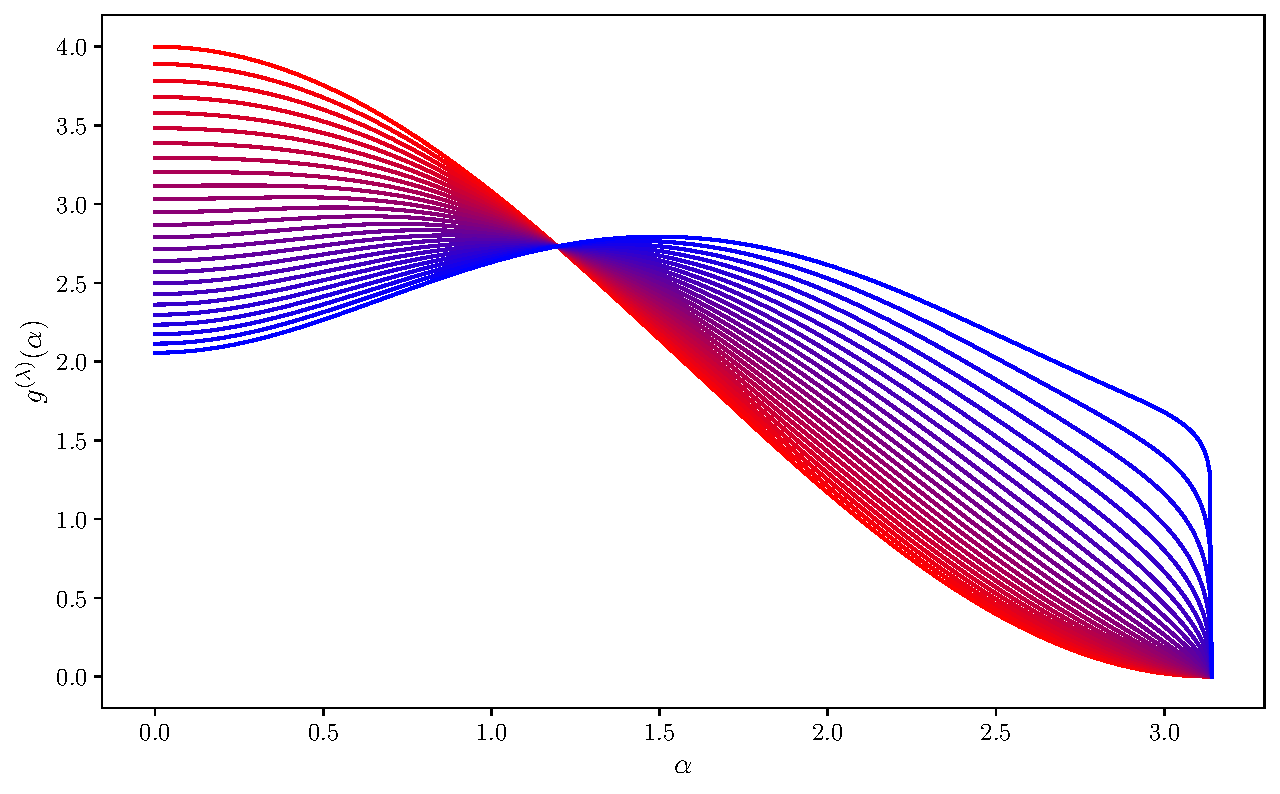
\includegraphics[width=10cm]{family_curves_g.pdf}
        \vspace{-4mm}
    	\mycaption{The curves of $\alpha\mapsto g^{(\lambda)}(\alpha)$ for the values $\lambda=\frac{i}{50}$ from $i=0$ (red) to $i=24$ (blue).}
    	\label{fig:family_curves_g}
    \end{figure}
    
    Writing $g(\alpha)=g_1(\alpha)^{\lambda}g_2(\alpha)^{1-2\lambda}$ for $g_1(\alpha)=6-2\cos(2\alpha)$ and $g_2(\alpha)=2+2\cos\alpha$, we compute the first derivative of $g$, and apply the double angle formulas $\cos(2\alpha)=2\cos^2\alpha-1$ and $\sin(2\alpha)=2\cos\alpha\sin\alpha$:
    \begin{align*}
         \frac{\dd}{\dd\alpha}g(\alpha)&=g_1(\alpha)^{\lambda-1}g_2(\alpha)^{-2\lambda}\left(\lambda g_2(\alpha)\frac{\dd}{\dd\alpha}g_1(\alpha)+(1-2\lambda)g_1(\alpha)\frac{\dd}{\dd\alpha}g_2(\alpha)\right)\\
         &=g_1(\alpha)^{\lambda-1}g_2(\alpha)^{-2\lambda}\left(\lambda(2+2\cos\alpha)\cdot4\sin(2\alpha)+(1-2\lambda)(6-2\cos(2\alpha))(-2\sin\alpha)\right)\\
         &=g_1(\alpha)^{\lambda-1}g_2(\alpha)^{-2\lambda}\left(\lambda(2+2\cos\alpha)\cdot4\cdot2\cos\alpha\sin\alpha+(1-2\lambda)\left(8-4\cos^2\alpha\right)(-2\sin\alpha)\right)\\
         &=8g_1(\alpha)^{\lambda-1}g_2(\alpha)^{-2\lambda}\sin\alpha\left(2\lambda \cos\alpha(1+\cos\alpha)-(1-2\lambda)\left(2-\cos^2\alpha\right)\right)\\
         &=8g_1(\alpha)^{\lambda-1}g_2(\alpha)^{-2\lambda}\sin\alpha\left(\cos^2\alpha+2\lambda\cos\alpha+4\lambda-2\right).
    \end{align*}
    
    The only interesting zeros of $\frac{\dd}{\dd\alpha}g(\alpha)$ are those of the last factor 
    $\cos^2\alpha+2\lambda\cos\alpha+4\lambda-2$: the factor $8g_1(\alpha)^{\lambda-1}g_2(\alpha)^{-2\lambda}$ has none, and those for $\sin\alpha$ are $\alpha=0$ and $\alpha=\pi$, with corresponding values $g(0)=2^{2-2\lambda}$ and $g(\pi)=0$.
    
    Our first claim is that the equation $\mathcal E:\cos^2\alpha+2\lambda\cos\alpha+4\lambda-2=0$ has a unique solution $\cos\alpha=-\lambda+\sqrt{\lambda^2-4\lambda+2}$ if $\lambda\geq 1/6$ and has no solution $\cos\alpha$ otherwise. To see this, we consider $\mathcal E$ as an equation of second degree in $\cos\alpha$, which leads to the two solution candidates $\cos\alpha=-\lambda\pm\sqrt{\lambda^2-4\lambda+2}$.
     
    We can exclude the solution $\cos\alpha=-\lambda-\sqrt{\lambda^2-4\lambda+2}$ since $\cos\alpha\in[-1,1]$ and $\lambda\in [0,1/2)$. 
    The other solution needs to be excluded for the same reason if $\lambda<1/6$.

    Our second claim is that $\frac{\dd^2}{\dd^2\alpha}g(\alpha)\vert_{\alpha=0}$ has the same sign as $6\lambda -1$. To see why, we apply the definition of the second derivative:
    \begin{align*}
        \frac{\dd^2}{\dd^2\alpha}g(\alpha)\vert_{\alpha=0}
        &=\lim_{\alpha\to 0}\frac{\frac{\dd}{\dd\alpha}g(\alpha)}{\alpha}\\
        &=\lim_{\alpha\to 0}8(6-2\cos(2\alpha))^{\lambda-1}(2+2\cos\alpha)^{-2\lambda}\cdot\frac{\sin\alpha}{\alpha}\cdot\left(\cos^2\alpha+2\lambda\cos\alpha+4\lambda-2\right)\\
        &=8\cdot4^{\lambda-1}\cdot 4^{-2\lambda}\cdot 1\cdot(6\lambda -1)\\
        &=2^{1-2\lambda}(6\lambda -1).
    \end{align*}
    
    Therefore, in case $\lambda<1/6$, we can conclude from the two claims that $g(\alpha)$ reaches its maximum at $\alpha_0=0$, and this maximum is then equal to $2^{2-2\lambda}=2^{2\mu}$, as required. For $\lambda=1/6$, the solution to the equation $\mathcal E$ is $\cos\alpha=1$, again implying that $g(\alpha)$ reaches its maximum at $\alpha_0=0$, and we obtain the same maximum of $2^{2\mu}$. In case $\lambda>1/6$, the two claims imply that $g(\alpha)$ reaches its maximum at the unique $\alpha_0\in[0,\pi]$ for which $\cos\alpha_0=-\lambda+\sqrt{\lambda^2-4\lambda+2}$. For this $\alpha_0$, the double angle formula for the cosine implies that $\cos(2\alpha_0)=4\lambda^2-8\lambda+3-4\lambda\sqrt{\lambda^2-4\lambda+2}$. If we replace $\cos\alpha_0$ and $\cos(2\alpha_0)$ by their respective values, we obtain that the maximum of $g(\alpha)$ for $\alpha\in[0,\pi]$ is given by the following value:
    \[
        g(\alpha_0)=\frac{\left(-8\lambda^2+16\lambda+8\lambda\sqrt{\lambda^2-4\lambda+2}\right)^{\lambda}}{\left(2-2\lambda+2\sqrt{\lambda^2-4\lambda+2}\right)^{2\lambda-1}}=2^{2\mu}.
    \]
    With this, we have covered the case $(p,q,r;u,v)=(t,0,0;n-2t,0)$ entirely. Similarly, it can be proven that $|P_{t,a}(z)|$ is also bounded by $2^{\mu n}$ on $\dis$ for the remaining two cases of $(p,q,r;u,v)$. 
    For $(p,q,r;u,v)=(0,t,0;n-2t,0)$, one can proceed in exactly the same way, and for $(p,q,r;u,v)=(0,0,t;n-2t,0)$, it is enough to replace $g(\alpha)$ by $h(\alpha)=(2+2\cos(2\alpha))^\lambda(2+2\cos\alpha)^{1-2\lambda}$, whose maximum is bounded by the maximum of $g(\alpha)$ since $0\leq h(\alpha)\leq g(\alpha)$.
\end{proof}

The curve of $\lambda\mapsto\mu(\lambda)$ defined in the above Theorem~\ref{theorem:bound_D_nka_generalized} is represented in Figure~\ref{fig:curve_exponents_lambda_mu}. Observe that $\mu(1/2)=3/4$, which corresponds to Theorem~\ref{theorem:bound_D_nka}.

\begin{figure}[ht]
	\centering
	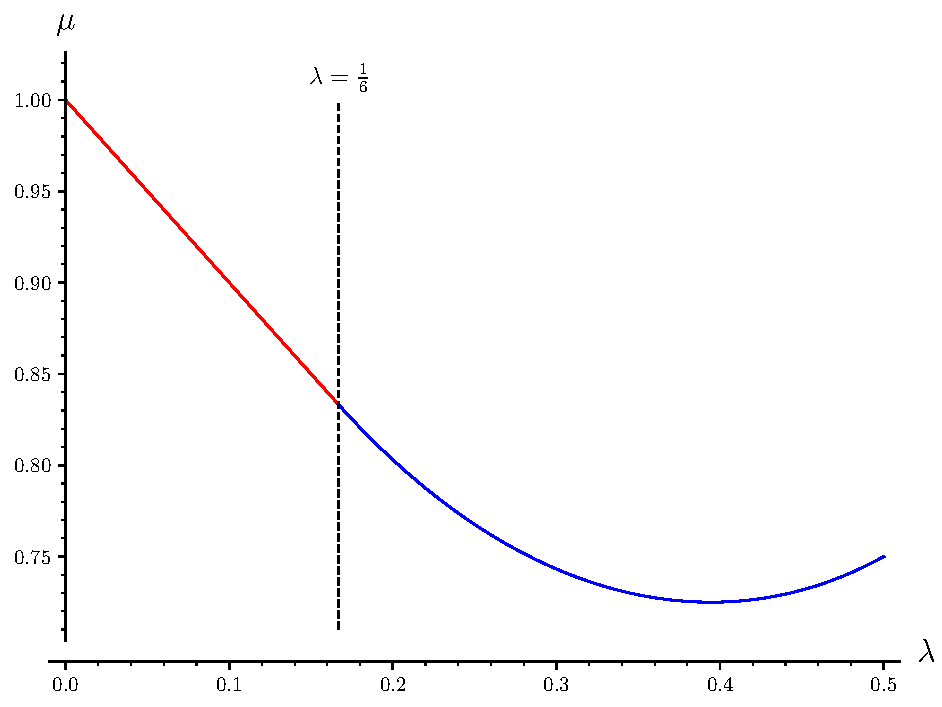
\includegraphics[width=9.5cm]{curve_exponents_lambda_mu.pdf}
    \vspace{-5mm}
	\mycaption{The curve of $\lambda\mapsto\mu(\lambda)$ with $0\leq\lambda\leq\frac 12$ from Theorem~\ref{theorem:bound_D_nka_generalized}.}
	\label{fig:curve_exponents_lambda_mu}
\end{figure}

\section{Experiments and comparisons}\label{sec:expAndComp}

In this section, we establish a tighter bound on the absolute value of the Walsh transform of the revisited \hwbf{} for even $n\in[1,80]$. 
We then compare the nonlinearity of this function to that of other functions suited to similar use cases, such as the \hwbf{} or the weightwise cyclic functions from~\cite{DAM:MeaOza24}.

\subsection{Bounding the Walsh transform of $f$ experimentally}\label{sec:expwt}

Following Corollary~\ref{cor:bound_walsh_cauchy}, we deduce that $|\wt f(a)|\leq 1+n\cdot 2^{3n/4}$ for every even integer $n\geq 0$ and every binary vector $a\in\F_2^n$, where $f\in\BN$ denotes the revisited \hwbf{}. This is a somewhat pessimistic bound. In this part, we discuss how a tighter bound on $|\wt f(a)|$ can be obtained in polynomial time in $n$.

This method is based on the identity given in Proposition~\ref{prop:WT}.
For this, consider a vector $b\in\mathbb F_2^n$; we write $(p,q,r)=(p(b),q(b),r(b))$. Also, for $k\in[1,n]$, let $b_k=b+\pi(e_k)$ and $(p_k,q_k,r_k)=(p(b_k),q(b_k),r(b_k))$, where $\pi:[1,n]\to[1,n]$ is again the permutation sending the first $n/2$ elements to the odd positions and the $n/2$ last ones to the even positions. Notice first that for every integer $k\in[1,n]$, it holds that $(p_k,q_k,r_k)\in\{(p\pm1,q,r\mp 1),(p,q\pm 1,r\mp 1)\}$. Furthermore, observe that if $k\in[0,n/2]$ and $(p_k,q_k,r_k)=(p+\alpha,q+\beta,r+\gamma)$ for $\{\alpha,\beta,\gamma\}=\{0,\pm 1\}$ with $\gamma\neq 0$, then we have $(p_{k+n/2},q_{k+n/2},r_{k+n/2})=(p+\alpha',q+\beta',r+\gamma')$ for some $\{\alpha',\beta',\gamma'\}=\{0,\pm 1\}$ with $\gamma'\neq 0$ which only depend on $\alpha$, $\beta$ and $\gamma$. Explicitly, we have $(\alpha',\beta',\gamma')=(\alpha,\beta,\gamma)$ if $\gamma=1$ and $(\alpha',\beta',\gamma')=(\beta,\alpha,\gamma)$ if $\gamma=-1$.

In the following discussion, we outline a method to determine an upper bound on $\max_{a\in\F_2^n}\wt f(a)$. A similar approach can be applied to find a lower bound on $\min_{a\in\F_2^n}\wt f(a)$, and by utilizing both, we can also obtain an upper bound on $\max_{a\in\F_2^n}|\wt f(a)|$ by making use of the following identity:
\[
	\max_{a\in\F_2^n}|\wt f(a)|=\max\Big(\max_{a\in\F_2^n}\wt f(a),-\min_{a\in\F_2^n}\wt f(a)\Big).
\]

For each $k\in[1,n/2]$, we select $\{\alpha_k,\beta_k,\gamma_k\}=\{0,\pm 1\}$ with $\gamma_k\neq 0$ such that the following expression, based on the notation introduced in Remark~\ref{rmk:Dnka_dep_pqr}, is defined and maximized:
\[
	B_k^{p,q,r}=\mathsf D_{k,n}^{p+\alpha_k,q+\beta_k,r+\gamma_k}+\mathsf D_{k+n/2,n}^{p+\alpha_k',q+\beta_k',r+\gamma_k'}.
\]
This implies that $\Dnka{n}{k}{b_k}+\Dnka{n}{k+n/2}{b_{k+n/2}}\leq B_k^{p,q,r}$ for every $k\in[1,n/2]$, leading to the conclusion that $\sum_{k=1}^n\Dnka nk{b_k}\leq\sum_{k=1}^{n/2} B_k^{p,q,r}$. As a result, we derive the following upper bound:
\begin{equation}\label{eqn:bound_walsh}
	\max_{a\in\F_2^n}\wt f(a)\leq 1+\max_{p+q+r=n/2}\sum_{k=1}^{n/2} B_k^{p,q,r}.
\end{equation}

Under the assumption that the values of $\mathsf{D}_{k,n}^{p,q,r}$ have already been computed for all $k\in[1,n]$ and for all triplets $(p,q,r)$ satisfying $p+q+r=n/2$, the bound in equation (\ref{eqn:bound_walsh}) can be determined with a computational complexity of $\mathcal{O}(n^3)$. This is because there are $\mathcal{O}(n^2)$ possible triplets $(p,q,r)$ that meet the condition $p+q+r=n/2$, and the summation itself can be computed in $\mathcal{O}(n)$ steps.

We consider now the complexity involved in computing the values of $\mathsf{D}_{k,n}^{p,q,r}$ for all $k\in[1,n]$ and all triplets $(p,q,r)$ satisfying $p+q+r=n/2$. We claim that this computation has a complexity of $\mathcal{O}(n^3 \log n)$. Towards this, it is sufficient to expand $(-z^2 + 2z + 1)^p \cdot (-z^2 - 2z + 1)^q \cdot (z^2 + 1)^r$ for all triplets $(p,q,r)$ such that $p+q+r=n/2$; this is due to Proposition \ref{proposition:generating_fct}.

To achieve this, we first precompute the expanded polynomial $(-z^2 + 2z + 1)^p$ for each $p\in[0,n/2]$. This can be done recursively using the formula $(-z^2 + 2z + 1)^{p+1} = (-z^2 + 2z + 1) \cdot (-z^2 + 2z + 1)^p$. For each $p$, this requires $\mathcal O(n)$ arithmetic computations. Performing this for every $p$ results in a total complexity of $\mathcal{O}(n^2)$. The same approach can be used to expand the polynomials $(-z^2 - 2z + 1)^q$ and $(z^2 + 1)^r$, resulting in an overall complexity of $\mathcal{O}(n^2)$ for all $p,q,r\in[0,n/2]$. 

Finally, for each triplet $(p,q,r)$ satisfying $p+q+r=n/2$, we multiply the three expanded polynomials $(-z^2 + 2z + 1)^p$, $(-z^2 - 2z + 1)^q$ and $(z^2 + 1)^r$. These two multiplications are performed in $\mathcal{O}(n \log n)$ operations by using the fast Fourier transform. Given that there are $\mathcal{O}(n^2)$ triplets $(p,q,r)$ to consider, we conclude that precomputing the values $\mathsf{D}_{k,n}^{p,q,r}$ for all $k\in[1,n]$ and all triplets $(p,q,r)$ has a complexity of $\mathcal{O}(n^3 \log n)$, making the overall complexity of the procedure also $\mathcal{O}(n^3 \log n)$.

\bigskip

In Table~\ref{table:max_walsh_vs_bound}, we compare the exact values of $\max_{a\in\mathbb F_2^n}|\wt f(a)|$ for small values of $n$ (calculated using \textsf{SageMath}) to the bound $B_n$ obtained through the above method and to the bound from Corollary~\ref{cor:bound_walsh_cauchy}. Additionally, Table~\ref{table:walsh_bounds} provides the values of the bound $B_n$ for all even values of $n\in[1,80]$. The method described above offers a tighter bound compared to Corollary~\ref{cor:bound_walsh_cauchy}. Its polynomial complexity makes it possible to extend the analysis well beyond the limitations imposed by a full computation of the Walsh spectrum, which requires a complexity of $\mathcal O(n2^n)$.
\ifnum\anon=0
	We provide a \textsf{SageMath} implementation to obtain the bound $B_n$: \url{https://github.com/se-tim/Revisited-HWBF.git}.
\fi

\begin{table}[ht]
	\small
	\centering
	\begin{tabular}{|c|c|c|c|}
		\hline
		$n$ & $\max_{a\in\F_2^n}|\wt f(a)|$ & $B_n$  & $\lfloor 1+n \cdot 2^{3n/4} \rfloor$\\ \hline
		$2$  & $2$     & $2$  &  $6$ \\
		$4$  & $8$     & $8$  & $33$  \\
		$6$  & $20$    & $28$   & $136$\\
		$8$  & $52$    & $76$  & $513$ \\
		$10$ & $108$   & $212$  & $1\,811$\\
		$12$ & $292$   & $596$  & $6\,145$ \\
		$14$ & $700$   & $1\,828$ & $20\,275$ \\
		$16$ & $2\,176$  & $5\,196$ & $65\,537$ \\
		$18$ & $4\,964$  & $14\,668$ & $208\,535$ \\
		$20$ & $14\,968$ & $41\,468$ & $655\,361$ \\
		$22$ & $34\,232$ & $118\,544$ & $2\,039 \,002$ \\
		$24$ & $109\,648$ & $325\,188$ & $6\,291 \,457$  \\ \hline
	\end{tabular}
	\mycaption{The actual $\max_{a\in\F_2^n}|\wt f(a)|$ compared to the bound $B_n$ and the theoretical bound from Corollary~\ref{cor:bound_walsh_cauchy}.}
	\label{table:max_walsh_vs_bound}
\end{table}

\begin{table}[ht]
	\small
	\centering
	\begin{minipage}{0.24\textwidth}
		\centering
		\begin{tabular}{|c|c|}
			\hline
			$n$ & $\approx B_n$ \\
			\hline
			$2$  & $2.00 \cdot 10^{0}$  \\
			$4$  & $8.00 \cdot 10^{0}$  \\
			$6$  & $2.80 \cdot 10^{1}$  \\
			$8$  & $7.60 \cdot 10^{1}$  \\
			$10$ & $2.12 \cdot 10^{2}$  \\
			$12$ & $5.96 \cdot 10^{2}$  \\
			$14$ & $1.83 \cdot 10^{3}$  \\
			$16$ & $5.20 \cdot 10^{3}$  \\
			$18$ & $1.47 \cdot 10^{4}$  \\
			$20$ & $4.15 \cdot 10^{4}$  \\
			\hline
		\end{tabular}
	\end{minipage}%
	\begin{minipage}{0.24\textwidth}
		\centering
		\begin{tabular}{|c|c|}
			\hline
			$n$ & $\approx B_n$ \\
			\hline
			$22$ & $1.19 \cdot 10^{5}$  \\
			$24$ & $3.25 \cdot 10^{5}$  \\
			$26$ & $9.59 \cdot 10^{5}$  \\
			$28$ & $2.68 \cdot 10^{6}$  \\
			$30$ & $7.65 \cdot 10^{6}$  \\
			$32$ & $2.14 \cdot 10^{7}$  \\
			$34$ & $6.25 \cdot 10^{7}$  \\
			$36$ & $1.76 \cdot 10^{8}$  \\
			$38$ & $5.03 \cdot 10^{8}$  \\
			$40$ & $1.40 \cdot 10^{9}$  \\
			\hline
		\end{tabular}
	\end{minipage}%
	\begin{minipage}{0.24\textwidth}
		\centering
		\begin{tabular}{|c|c|}
			\hline
			$n$ & $\approx B_n$ \\
			\hline
			$42$ & $4.01 \cdot 10^{9}$  \\
			$44$ & $1.12 \cdot 10^{10}$ \\
			$46$ & $3.21 \cdot 10^{10}$ \\
			$48$ & $8.91 \cdot 10^{10}$ \\
			$50$ & $2.56 \cdot 10^{11}$ \\
			$52$ & $7.12 \cdot 10^{11}$ \\
			$54$ & $2.05 \cdot 10^{12}$ \\
			$56$ & $5.73 \cdot 10^{12}$ \\
			$58$ & $1.65 \cdot 10^{13}$ \\
			$60$ & $4.59 \cdot 10^{13}$ \\
			\hline
		\end{tabular}
	\end{minipage}%
	\begin{minipage}{0.24\textwidth}
		\centering
		\begin{tabular}{|c|c|}
			\hline
			$n$ & $\approx B_n$ \\
			\hline
			$62$ & $1.32 \cdot 10^{14}$ \\
			$64$ & $3.66 \cdot 10^{14}$ \\
			$66$ & $1.05 \cdot 10^{15}$ \\
			$68$ & $2.93 \cdot 10^{15}$ \\
			$70$ & $8.40 \cdot 10^{15}$ \\
			$72$ & $2.33 \cdot 10^{16}$ \\
			$74$ & $6.71 \cdot 10^{16}$ \\
			$76$ & $1.87 \cdot 10^{17}$ \\
			$78$ & $5.39 \cdot 10^{17}$ \\
			$80$ & $1.51 \cdot 10^{18}$ \\
			\hline
		\end{tabular}
	\end{minipage}
	\mycaption{Approximate values of $B_n$ for various values of $n$.}
	\label{table:walsh_bounds}
\end{table}

\subsection{Comparison of the nonlinearity}

In this part, we compare the nonlinearity of the revisited \hwbf{} to other weightwise quadratic functions considered for similar use-cases, such as the majority function, the \hwbf{} and the cyclic weightwise functions studied in~\cite{DAM:MeaOza24}. 

In Figure~\ref{fig:walsh_bound_comparison}, we compare bounds for the values of $\max_{a \in \mathbb{F}_2^n} |\wt f(a)|$ for various functions $f\in\BN$, where a smaller maximum indicates better nonlinearity, see Definition~\ref{def:nl}.
We present values for $n$ up to $80$, which is sufficient for examining the asymptotic behavior of the different bounds.
The pink and orange curves represent the upper bounds  in~\cite{DAM:MeaOza24}, with the orange curve mostly overlapping the pink one. To go into more detail, the pink curve corresponds to the bound that holds for all cyclic weightwise linear functions $f$ that, with the notation from Definition~\ref{def:wwdegd}, satisfy $ f_0(x) = b \cdot x $ for $\w(b)$ odd; therefore, this represents for instance an upper bound for the \hwbf{}. The orange curve corresponds to the bound for the cyclic weightwise quadratic function $f$ defined by $f_0(x) = x_1 + x_2 x_3$.
The blue curve applies to both the majority and \hwbf{} functions, whose exact nonlinearities are given in Property~\ref{prop:wwd1}. We use a single curve here because, on a logarithmic scale, the nonlinearity difference between these two functions is too small to distinguish between them.
For the revisited \hwbf{} introduced in Definition~\ref{def:revHWBF}, the red curve corresponds to the theoretical bound from Corollary~\ref{cor:bound_walsh_cauchy}, while the green curve represents the experimental results from Section~\ref{sec:expwt}.

\begin{figure}[ht]
	\centering
	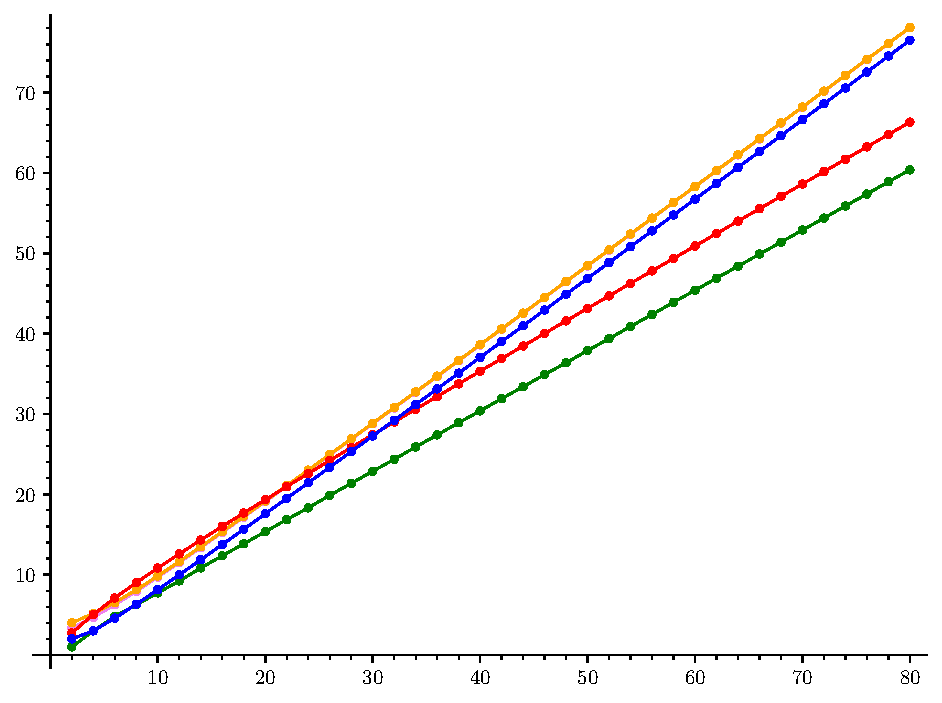
\includegraphics[width=10cm]{comparison_walsh_bound.pdf}
	\mycaption{
		Bounds on $\max_{a \in \mathbb{F}_2^n} |\wt f(a)|$ for various functions $f\in\BN$ and even values of $n$, shown on a logarithmic scale.
		The pink and orange curves, the orange one mostly covering the pink one, represent bounds for cyclic weightwise linear functions and a cyclic weightwise quadratic function from~\cite{DAM:MeaOza24}, respectively. The blue curve shows bounds for the majority function and the \hwbf{}. The theoretical bound for the revisited \hwbf{} (Corollary~\ref{cor:bound_walsh_cauchy}) is in red, and the experimental bound $B_n$ (Section~\ref{sec:expwt}) is in green.}
	\label{fig:walsh_bound_comparison}
\end{figure}

The revisited \hwbf{} demonstrates significantly better performance compared to the majority function, the original \hwbf{} and the functions studied in \cite{DAM:MeaOza24}. Its theoretical bound on $\max_{a \in \mathbb{F}_2^n} |\wt f(a)|$ reveals an asymptotic slope of $3/4$ on a logarithmic scale, contrasting with the slope of $1$ for the majority function, the \hwbf{}, and the bounds proven in~\cite{DAM:MeaOza24}. Notably, the green curve corresponding to the bound of Section~\ref{sec:expwt} appears to share this asymptotic slope of $3/4$, supporting the effectiveness of Corollary~\ref{cor:bound_walsh_cauchy} and the stronger Theorem~\ref{theorem:bound_D_nka_generalized} in capturing asymptotic behavior.

\bigskip

We also compare in Table~\ref{table:comparisonsNL} the precise nonlinearity values of the functions under consideration. Among the various weightwise quadratic functions studied so far, we observe that the revisited \hwbf{} has the highest nonlinearity from $n=10$ onward.

\begin{table}[ht]
	\small
	\centering
	\begin{tabular}{|c| c|c|c|c| c|c|c|}
		\hline
		$n$ & $4$  & $6$  & $8$  &  $10$ & $12$ & $14$ & $16$  \\
		\hline	
		\hwbf{}   & $4$  & $20$  & $88$  &  $372$ & $1\,544$ & $6\,344$ & $25\,904$  \\  	
		Majority   & $5$  & $22$  & $93$  &  $386$ & $1\,586$ & $6\,476$ & $26\,333$  \\
		$t$~\cite{DAM:MeaOza24}   & $4$  & $22$  & $96$  &  $404$ & $1\,672$ & $6\,854$ & $27\,884$\\
		$u$~\cite{DAM:MeaOza24}   & $4$  & $24$  & $104$  &  $456$ & $1\,888$ & $7\,816$ & $31\,616$ \\
		Revisited \hwbf{}  & $4$  & $22$  & $102$  &  $458$ & $1\,902$ & $7\,842$ & $31\,680$\\
\hline
	\end{tabular}
	\mycaption{Comparison of the nonlinearity.}
	\label{table:comparisonsNL}
\end{table}

\section{Other parameters}\label{sec:otherParameters}

In this section, we present additional cryptographic parameters for the revisited \hwbf{}. While Theorem~\ref{th:bal} describes its balancedness and Sections~\ref{sec:Cauchy} and \ref{sec:expAndComp} thoroughly explore its nonlinearity, our focus here will be on its algebraic characteristics. Specifically, we will examine the degree, the algebraic immunity, and the fast algebraic immunity, and offer comparisons with other weightwise quadratic functions.

\begin{proposition}
	Let $n\geq 4$ be even, and let $f\in\BN$ be the revisited \hwbf{}. Then $\degg(f)=n-1$.
\end{proposition}
\begin{proof}
	We write $f=q+h$, where $q\in\BN$ is given by $q(x)=\sum_{i=1}^{n/2} (x_i+1) x_{i+n/2}$ and $h\in\BN$ is the \hwbf{}.
	The function $h$ has degree $n-1\geq 3$ by Property~\ref{prop:wwd1}, and the function $q$ has no monomial of degree higher than $2$, so that $\degg(f)=\degg(h)=n-1$.
\end{proof}

In Table~\ref{table:comparisonsDeg}, we display the algebraic degree of different weightwise quadratic function. We observe that the revisited \hwbf{} is the function with the highest degree, together with the \hwbf{}. 

\begin{table}[ht]
	\small
	\centering
	\begin{tabular}{|c|c|c|c|c|c|c|c|}
		\hline
		$n$ & $4$  & $6$  & $8$  &  $10$ & $12$ & $14$ & $16$  \\
		\hline
		\hwbf{}   & $3$  & $5$  & $7$  &  $9$ & $11$ & $13$ & $15$  \\  	
		Majority   & $4$  & $4$  & $8$  &  $8$ & $8$ & $8$ & $16$  \\
		$t$~\cite{DAM:MeaOza24}   & $2$  & $5$  & $6$  &  $9$ & $11$ & $13$ & $14$\\
		$u$~\cite{DAM:MeaOza24}   & $2$  & $4$  & $6$  &  $8$ & $10$ & $12$ & $14$ \\
		Revisited \hwbf{}  & $3$  & $5$  & $7$  &  $9$ & $11$ & $13$ & $15$\\
		\hline
	\end{tabular}
	\mycaption{Comparison of the degree.}
	\label{table:comparisonsDeg}
\end{table}

\begin{proposition}
	Let $n\geq 4$ be even, let $f\in\BN$ be the revisited \hwbf{}, and let $h\in\BN$ be the \hwbf{}. Then the following holds:
	\[\AI(f)\geq \AI(h)-2.\]
\end{proposition}

\begin{proof}
	Let $q\in\BN$ be given by $q(x)=\sum_{i=1}^{n/2} (x_i+1) x_{i+n/2}$, so that $h=f+q$.
	Let $g\in\BN^*$ with $\degg(g)=\AI(f)$ be an annihilator of $f+ \varepsilon$ for some $\varepsilon\in\{0,1\}$. 
	Then the following holds:
	\[g\cdot(q+1) \cdot(h+\varepsilon) = g\cdot(q+1)\cdot(f+q+\varepsilon)=g\cdot(q+1)\cdot(f+\epsilon)+g\cdot(q+1)\cdot q=0+0=0.\]
	Hence, $g\cdot(q+1)$ is an annihilator of $h+ \varepsilon$. 
	If $g\cdot(q+1)\ne 0$, it follows that $\AI(h)\leq\degg(g\cdot(q+1))\leq\degg(g)+\degg(q+1)$, and therefore that $\AI(f)=\degg(g)\geq\AI(h)-\degg(q+1)=\AI(h)-2$. If $g\cdot(q+1)=0$, then $0=g\cdot(f+\epsilon+q+1)=g\cdot(h+\epsilon+1)$, showing that $\AI(f)=\degg(g)\geq\AI(h)$.
\end{proof}

From Theorem 4 in~\cite{DAM:WCST14}, the algebraic immunity of the \hwbf{} is at least $\lfloor n/3\rfloor +1$, which leads to $\lfloor n/3\rfloor -1$ for the revisited \hwbf{}.
In Table~\ref{table:comparisonsAI}, we present the algebraic immunity of various weightwise quadratic functions. We observe that the revisited \hwbf{} demonstrates the best performance after the majority function; the latter is known to achieve optimal algebraic immunity.

\begin{table}[ht]
	\small
	\centering
	\begin{tabular}{|c| c|c|c|c| c|c|c|}
		\hline
		$n$ & $4$  & $6$  & $8$  &  $10$ & $12$ & $14$ & $16$  \\
		\hline	
		\hwbf{}   & $2$  & $3$  & $4$  &  $4$ & $5$ & $5$ & $6$  \\  	
		Majority   & $2$  & $3$  & $4$  &  $5$ & $6$ & $7$ & $8$  \\
		$t$~\cite{DAM:MeaOza24}   & $2$  & $3$  & $4$  &  $5$ & $5$ & $6$ & $7$\\
		$u$~\cite{DAM:MeaOza24}   & $2$  & $3$  & $4$  &  $5$ & $6$ & $6$ & $7$ \\					
		Revisited \hwbf{}   & $2$  & $3$  & $4$  &  $5$ & $6$ & $6$ & $7$\\
		\hline
	\end{tabular}
	\mycaption{Comparison of the algebraic immunity.}
	\label{table:comparisonsAI}
\end{table}

Lastly, we also considered the fast algebraic immunity of the revisited \hwbf{} $f$. In Table~\ref{table:FAI}, we give the best couples $(d,e)$ encountered for the function $f$, where $\degg(g)=d$ and $\degg(h)=e$ for functions $g$ and $h$ satisfying $fg=h$.

\bigskip

These various results on the algebraic properties of the revisited \hwbf{} suggest that it possesses strong resistance against standard attacks. Furthermore, its high nonlinearity makes it a well-suited candidate for use as a filter function in contexts such as filtered \textsf{LFSR}s or in homomorphically-friendly schemes like \textsf{FLIP} and \textsf{FiLIP}.

\begin{table}[ht]
	\small
	\centering
	\begin{tabular}{|c|c|c|c|c|c|c|c|c|}
		\hline
		$ n $      & $4$     & $6$     & $8$     & $10$    & $12$    & $14$    & $16$    & $18$    \\ \hline
		$(d, e)$ & $(1,2)$ & $(1,3)$ & $(1,5)$  & $(1,7)$ & $(1,9)$ & $(1,11)$ & $(1,13)$ & $(1,15)$ \\ 
		&     &    & $(2,4)$  & $(2,6)$ & $(2,8)$ & $(2,10)$ & $(2,12)$ & $(2,14)$\\ 
		&     &    &     & $(3,5)$ & $(3,6)$ & $(3,9)$ & $(3,11)$ & $(3,13)$\\ 
		&     &    &     &  &  &  & $(4,9)$ & $(4,11)$\\ 
	 	&     &    &     &  &  &  &  & $(5,10)$ \\ \hline
	\end{tabular}
	\mycaption{Lowest possible values of $(d, e)$ for different values of $n$.}
	\label{table:FAI}
\end{table}

\section{Conclusion and open questions}

In this work, we introduced the revisited hidden weight bit function, a weightwise quadratic Boolean function with improved cryptographic properties over existing constructions. 
We analyzed its balancedness, and using generating functions in combination with complex analysis, we derived interesting lower bounds on its nonlinearity, demonstrating that the revisited \hwbf{} achieves superior nonlinearity compared to other functions with similar computational costs. 
We further examined other cryptographic parameters such as degree, algebraic immunity, and fast algebraic immunity, confirming that the revisited \hwbf{} matches or outperforms comparable functions in these aspects.

Our approach utilizes generating functions and Cauchy’s estimate to establish lower bounds on the nonlinearity of weightwise quadratic functions. 
This naturally raises the question: can the employed techniques, particularly the use of Cauchy’s estimate, be extended to other families of Boolean functions? Specifically, this approach appears feasible for other weightwise-degree-$d$ functions $f$ where the $f_k$ are direct sums. 
Investigating this could potentially lead to the discovery of new functions with comparable computational costs and even better cryptographic properties.

\ifnum\anon=0
	\section{Acknowledgments}
	Pierrick Méaux was funded by the European Research Council (\textsf{ERC}) under the Advanced Grant program (reference number: 787390). Tim Seuré acknowledges the support of the Luxembourgish “Fonds National de la Recherche” (\textsf{FNR}) through an Individual Grant (reference number: 17936291).
\fi

\newpage

\ifnum\full=0
	\bibliographystyle{splncs04}
	\bibliography{add}
\else
	\bibliographystyle{alpha}
	\bibliography{add}
\fi

\end{document}